%\documentclass[12pt]{article}
%\setlength{\textwidth}{167mm}
%\setlength{\headsep}{0mm}
%\setlength{\headheight}{0mm}
%\setlength{\textheight}{230mm}
%\setlength{\oddsidemargin}{1.6mm}
%\setlength{\evensidemargin}{1.6mm}
%\setlength{\topmargin}{4.6mm}
%
%\usepackage{chngcntr}
%\usepackage{xspace}
%\usepackage{color}
%\usepackage{graphicx}
%\usepackage{amsmath}	% Advanced maths commands
%\usepackage{amssymb}	% Extra maths symbols
%\usepackage{lscape}
%\usepackage{longtable}
%\usepackage{threeparttable}
%\usepackage{multirow}
%\usepackage[figurename={Supplementary Figure}, tablename={Supplementary Table}]{caption}
%\usepackage{booktabs}
%\usepackage[ ]{hyperref}
%\graphicspath{{Images/}}
%%\usepackage[symbol]{footmisc}
%
%
%% Astronomical abbreviations (thanks to Dan Huber)
%\newcommand{\numax}{\mbox{$\nu_{\rm max}$}\xspace}
%\newcommand{\dnu}{\mbox{$\Delta \nu$}\xspace}
%\newcommand{\muHz}{\mbox{$\mu$Hz}\xspace}
%\newcommand{\teff}{\mbox{$T_{\rm eff}$}\xspace}
%\newcommand{\logg}{\mbox{$\log(g)$}\xspace}
%\newcommand{\feh}{\mbox{$\rm{[Fe/H]}$}\xspace}
%\newcommand{\msun}{\mbox{$\mathrm{M}_{\odot}$}\xspace}
%\newcommand{\lsun}{\mbox{$\mathrm{L}_{\odot}$}\xspace}
%\newcommand{\mearth}{\mbox{$\mathrm{M}_{\oplus}$}\xspace}
%\newcommand{\rsun}{\mbox{$\mathrm{R}_{\odot}$}\xspace}
%\newcommand{\kepler}{\emph{Kepler}\xspace}
%\newcommand{\tess}{\emph{TESS}\xspace}
%\newcommand{\ktwo}{K2\xspace}
%\newcommand{\gaia}{\emph{Gaia}\xspace}
%
%\begin{document}

\section*{\underline{Supplementary Information}}
\tableofcontents

\section{Asteroseismic Model}\label{s:seismo}
In order to extract signatures of stellar rotation from the asteroseismic p mode frequencies, we built a model that simultaneously treats the convective background ($B(\nu)$), the oscillations ($O(\nu)$), and the white noise ($W$), where $\nu$ is frequency \cite{davies+2015}. Our data, observed with \kepler, are also subject to the apodization (attenuation) of signals in the frequency-domain, where we fit our model \cite{chaplin+2011}. The apodization in power is given by

\begin{equation}\label{eq:apodization}
	\eta^2(\nu) = \rm{sinc}^2\left(\frac{\pi}{2}\frac{\nu}{\nu_{\rm nyq}}\right)\, ,
\end{equation}
where $\nu_{\rm nyq}$ is the Nyquist frequency for the \kepler short cadence, which was treated as a free parameter in our model to account for gaps in the data. Apodization only affects signals with characteristic timescales, meaning that it does not affect the white noise level, only the oscillations and convective background components. Given the above, our comprehensive model for the power spectrum is

\begin{equation}\label{eq:model}
	M(\nu) = W + \eta^2(\nu)[O(\nu) + B(\nu)]\, .
\end{equation}

\subsection{Convective Background ($B(\nu)$)}
To model the convective background we used three Harvey components \cite{harvey1985}, which express the background in power as Lorentzian-like functions centered on zero frequency. The Harvey components take the form 

\begin{equation}
	H(\nu, a, b, x) = \frac{4a^2/b}{1 + (2\pi b\nu)^x}\, ,
\end{equation}

\noindent where $a$ and $b$ are the free parameters in our model, and $x$ is fixed. The three Harvey components together form our background function as

\begin{equation}\label{eq:background}
	B(\nu) = H(\nu, a, b, x=4) + H(\nu, c, d, x=4) + H(\nu, j, k, x=2)\, ,
\end{equation}

\noindent where we have labeled parameters for the separate components. The $x = 2$ term here contributes to the background at high frequencies, whereas the $x=4$ terms contribute the background at low frequencies.

\subsection{Modes of Oscillation ($O(\nu)$)}
Modes of oscillation appear in the power spectrum as Lorentzian peaks \cite{chaplin+basu2017}. These peaks can be described by three values: the radial order ($n$, the overtone number of the oscillation), the angular degree ($\ell$) and the azimuthal order ($m$). Due to stellar rotation, each mode with an angular degree of $\ell > 0$ is split into its $(2\ell +1)$ Lorentzian components, labeled by $m$. For all $\ell=(0,1,2)$ modes identified for our targets in the  `Kages'  and LEGACY studies \cite{davies+2016,lund+2017} we add a (set of) Lorentzian(s) to our model, building a composite model representing all visible modes. The construction of our oscillation model takes the form

\begin{equation}
	O(\nu) = \sum_n \sum_\ell \sum_{m=-\ell}^\ell \frac{H_{n,\ell,m}}{1 + \frac{4}{\Gamma^2_{n,\ell}}(\nu - \nu_{n,\ell,m})^2}\, ,
\end{equation}

\noindent where $H_{n,\ell,m}$ is the height of the mode, $\Gamma_{n,\ell}$ is the linewidth of the mode (approximated to be equal for all split azimuthal orders at a single $n$ and $\ell$) and $\nu_{n, \ell, m}$ is the frequency of the mode. The range of $n$ differs per star depending on how many radial orders were reported in LEGACY or Kages, and the range of $\ell$ depends on how many angular degrees were reported for the corresponding radial order.

\subsubsection{Mode Frequencies and Rotational Splitting ($\nu_{n,\ell,m}$)}\label{ssec:frequencies}
The mode frequencies of main sequence stars are described by the asymptotic expression \cite{tassoul1980, vrard+2016}. The asymptotic expression defines the locations of the modes as regularly spaced, with structured deviation around \numax, the frequency of maximum oscillation amplitude. The expression takes the form

\begin{equation}\label{eq:asymptotic}
	\nu_{n,\ell,m} = \dnu\left(n + \epsilon + \delta\nu_{0\ell} + \frac{\alpha}{2}(n - \frac{\numax}{\dnu} + \epsilon)^2\right) + m\nu_{s}\, ,
\end{equation}

\noindent where \dnu is the large frequency separation between two consecutive radial orders $n$, $\epsilon$ is a a phase offset, $\delta\nu_{0\ell}$ is the small frequency separation between two oscillation modes of different $\ell$ at the same radial order, $\alpha$ describes the curvature of the spacing around \numax, and $\nu_s$ is the rotational splitting. Note that here we have expressed the small separation $\delta\nu_{0\ell}$ as a fraction of $\dnu$. In order to improve the computational efficiency of this analysis, we fixed \dnu to the values reported in LEGACY and Kages.

Instead of calculating mode frequencies directly from Equation \ref{eq:asymptotic} for the model, we treated the individual mode frequencies as parameters as well, drawn from Equation \ref{eq:asymptotic}. This is called a `latent parameter' implementation \cite{hogg2012, hall+2019}, as it forms a step between the parameters we want to draw inference on (also called hyperparameters) and our data. 
The parameters $\nu_{n,\ell,m}$ were allowed to vary within an uncertainty $\sigma_{\ell}$, which has a single value for each angular degree and also varied as a free parameter.
This allowed us to account for small shifts in frequency due to sudden changes in the stellar structure \cite{mazumdar+2014}. 

The mode frequency latent parameters were drawn from a normal distribution using Equation \ref{eq:asymptotic} as its mean function, as

\begin{equation}
	\nu_{n, \ell, m} \sim \mathcal{N}(\nu_{n, \ell, m}, \sigma_{\ell})\, ,
\end{equation}

\noindent where the expression $\nu_{n, \ell, m}$ on the right hand side represents the contents of Equation \ref{eq:asymptotic}, and $\mathcal{N}$ represents a normal distribution with a mean equal to $\nu_{n, \ell, m}$ and a standard deviation equal to $\sigma_{\ell}$. The symbol `$\sim$' indicates that the parameters on the left hand side of the equation are drawn from the probability distribution on the right hand side. This notation will be used throughout this work.

\subsubsection{Mode Linewidth ($\Gamma_{n,\ell}$)}
The linewidths of asteroseismic p modes vary roughly as a function of mode frequency, and do so slowly relative to \dnu. This can be expressed as an empirical relation \cite{lund+2017, davies+2014, appourchaux+2016}. However, this relation has six free parameters, none of which are directly relevant to this work. Instead of fitting this relation, we chose to employ a more flexible Gaussian Process \cite[GP]{rasmussen+williams2006} to act as a prior on the linewidths. This can be considered as us modelling the linewidths as correlated measurements, effectively loosely constraining how linewidth varies with frequency.

A GP is defined by a covariance kernel (describing the degree of correlation between linewidths) and a mean function (describing a global trend with frequency). As this approach describes the mode linewidths relative to one another in frequency, the radial orders of each target $n$ were rescaled to be between 0 (for the lowest $n$) and 1 (for the highest $n$). The radial orders of $\ell = 2$ modes were increased by $1$ to ensure this approximation applied to all modes. This approximation was used to describe the change in linewidth as a function of frequency without depending on the exact frequencies of the modes, which themselves were free parameters (see above). Given this, we defined our GP covariance kernel as a Squared Exponential Kernel to capture the slight periodicity of linewidth with frequency, as

\begin{equation}\label{eq:gpkernel}
	K_{i,j} = \rho^2 \exp \left[ -\frac{(n_{\textrm{f}, i} - n_{\textrm{f}, j})^2}{2L^2} \right]\, ,
\end{equation}

\noindent where $n_{\rm f}$ is the fractional radial order of a given mode and  $K_{i,j}$ represents an element of the covariance matrix $\underline{K}$, describing the covariance between two values of linewidth at different fractional radial orders. The GP kernel has two hyperparameters: $\rho$, which determines the spread of the kernel in linewidth, and $L$, which determines the length scale in terms of $n_{\rm f}$. The length scale $L$ was significantly larger than the large frequency separation (\dnu) in all cases, and so we considered the use of fractional radial orders a valid approximation in this model.

A linear function was used for the mean of the GP, as

\begin{equation}\label{eq:gpmean}
	\mu = m \times n_{\textrm{f}} + c\, ,
\end{equation}
where $m$ and $c$ are the slope and intercept of the line. The linewidth latent parameters were then drawn from the multivariate probability distribution

\begin{equation}\label{eq:gammagp}
	\Gamma \sim \mathcal{N}(\mu, \underline{K})\, ,
\end{equation}

\noindent where $\Gamma$ represents the linewidths of all the modes in the model. The parameters $m$, $c$ and $\rho$ were marginalised over, whereas $L$ was fixed to a pre-determined value.

\subsubsection{Mode Heights and Angle of Inclination ($H_{n,\ell,m}$)}
The height in power of each mode, $H_{n, \ell, m}$, varies not only as a function of distance in frequency from \numax, but also due to observation conditions, such as inclination angle and passband. In our model, we treated $H_{n, \ell, m}$ as a deterministic parameter, as

\begin{equation}\label{eq:height}
	H_{n, \ell, m} =  \varepsilon_{\ell, m}(i) \frac{2 (A_{n, \ell})^2}{\pi \Gamma_{n, \ell}}\, ,
\end{equation}

\noindent where $\varepsilon_{\ell, m}(i)$ modulates the height as a function of inclination angle $i$ (see below), and $A_{n, \ell}$ and $\Gamma_{n, \ell}$ are the mode amplitude and linewidth respectively for a given radial order and angular degree. Instead of modeling and modulating height directly, we instead sampled in amplitude and linewidth. This approach mitigates the correlations between height and linewidth in the sampling process \cite{toutain+appourchaux1994}.

As done above for the mode frequencies and linewidths, the mode amplitudes $A_{n,\ell}$ were also treated as latent parameters drawn from a probability distribution governed by hyperparameters. For this, we used a Gaussian function $G(\nu)$, centered on $\numax$, as

\begin{equation}\label{eq:amplitude}
	G(\nu) = A \times \exp\left[-\frac{(\nu - \numax)^2}{2w^2}\right]\, ,
\end{equation}

\noindent where $A$ is the modes' amplitude at \numax, and $w$ is the width of the Gaussian, both free parameters in our model. 
The mode amplitude latent parameters were then drawn from the probability distribution

\begin{equation}\label{eq:amplitwod}
	A_{n, \ell} \sim \mathcal{N}(G(\nu_{n,\ell}) \times V_\ell, \sigma_{A})\, ,
\end{equation}

\noindent where $V_\ell$ is a free parameter for the mode visibility of different angular degrees, which should be consistent for all \kepler observations. These parameters describe the difference in relative height between modes of different radial order. The mode visibility for $V_0$ is fixed at 1, and $V_{1,2}$ are treated as free parameters. The parameter $\sigma_{A}$, the uncertainty on the distribution, is also a free parameter, and takes the same value for all amplitudes regardless of angular degree.\\

The angle of inclination of a star with respect to Earth changes the net perturbation by a given mode when integrated across the stellar disc, changing the amplitudes of modes of different azimuthal orders. This is a geometric problem, and is expressed by $\varepsilon_{\ell, m}(i)$, which takes the form \cite{gizon+solanki2003}

\begin{equation}\label{eq:legendre}
	\varepsilon_{\ell, m}(i) = \frac{(\ell - |m|)!}{(\ell + |m|)!}\left[P_\ell^{|m|}(\cos(i))\right]^2\, ,
\end{equation}

\noindent where $P_\ell^{|m|}$ are associated Legendre functions. For the first three angular degrees, Equation \ref{eq:legendre} takes the form \cite{handberg+campante2011}

\begin{equation}
	\begin{split}
		\varepsilon_{0,0}(i) &= 1\, ,\\
		\varepsilon_{1,0}(i) &= \cos^2(i)\, ,    \\
		\varepsilon_{1,\pm1}(i) &= \frac{1}{2}\sin^2(i)\, ,\\
		\varepsilon_{2,0}(i) &= \frac{1}{4}(3\cos^2(i) - 1)^2\, ,\\
		\varepsilon_{2,\pm1}(i) &= \frac{3}{8}\sin^2(2i)\, ,\\
		\varepsilon_{2,\pm2}(i) &= \frac{3}{8}\sin^4(i)\, ,
	\end{split}
\end{equation}

\noindent where the sum of available components for a single $\ell$ are normalized to one.

\subsection{Likelihood Function for $M(\nu)$}\label{sec:like}
If data have Gaussian noise in the time domain, they will appear in the frequency domain with noise following a $\chi^2$ distribution with two degrees of freedom \cite[$\chi^2_2$ hereafter]{appourchaux+1998}. The noise properties of $\chi^2_2$ distributed data are multiplicative, and require a specific treatment when fitting a model. As our frequency bins can be approximated to be independent, we used the likelihood function \cite{anderson+1990},

\begin{equation}
	\ln p(\mathcal{P} | M(\nu)) = \sum_{j=0}^{N-1} \left[\ln[M_j(\nu)] + \frac{\mathcal{P}_j}{M_j(\nu)}\right]\, , 
\end{equation}

\noindent where $\mathcal{P}$ is the power spectral density (and thus our data), and $M(\nu)$ represents our model. The subscript $j$ denotes an individual datum, for a total of $N$ data. We have omitted the dependence of the model $M(\nu)$ on its parameters, for clarity. This equation is functionally equivalent to the evaluation of a gamma distribution of the form $\gamma(\mathcal{P} | 1, \beta)$, where $\beta = 1/M(\nu)$, which is the implementation we used in the sampling process.

\subsection{Model preparation and hyperparameter priors}
\subsubsection{Fitting the convective background}\label{sec:background}
Fitting the convective background, apodization and white noise component must be done for the full range of the power spectrum in order to be accurately constrained. However, fitting a single model to the full range of frequencies is computationally inefficient when we are interested in the modes of oscillation, as these occupy a relatively small range of frequencies.

In order to speed up this process, the background was first fit independently to a subset of our data for each star. This subset was created by removing all frequencies within a range $0.1 \times \dnu$ below and above the minimum and maximum mode frequencies reported in LEGACY and Kages. For KIC 3427720 we also removed frequencies in the range $90\, \mu\rm{Hz} < \nu < 400\, \mu{\rm{Hz}}$, where there were large peaks not of asteroseismic origin, skewing the background fit.

For each star the model function (see Eq. \ref{eq:model}) was fit, as

\begin{equation}
	M_{B}(\nu) = W + \eta^2(\nu)B(\nu)\, ,
\end{equation}

\noindent where $B(\nu)$ is the background model described in Equation \ref{eq:background}. The parameter components of our background fit are then $\phi_B = \{\log(a), \log(b), \log(c), \log(d), \log(j), \log(k), W, \nu_{\rm nyq}\}$, where the parameters of the Harvey components were sampled in log space. The model was fit to the background data using \texttt{PyStan} \cite{vanhoey+2013}, run for 10,000 iterations on each star. 

\subsubsection{Obtaining First Guesses and Prior Values}
In order to utilise some of the prior measurements of our targets without using them as hard constraints on our parameters, some of our model equations were fit to LEGACY and `Kages' data to obtain first guesses and mean values on hyperparameter priors.

For first guesses for parameters in the asymptotic expression, we fit Equation \ref{eq:asymptotic}, \textit{not} including the rotational component $m\nu_s$, to the $\ell = (0, 1, 2)$ mode frequencies reported in LEGACY and `Kages' for each star, using their reported uncertainties. This yielded estimates of $\hat{\epsilon}$, $\widehat{\delta\nu}_{01}$, $\widehat{\delta\nu}_{02}$ and $\hat{\alpha}$, where the hat symbol `\, $\widehat{}$\, ' indicates a prior value (e.g. $\hat{\nu}_{\rm max}$ is taken from LEGACY or `Kages'). While not precise, as we did not mitigate any perturbations due to acoustic glitches, these rough results act as functional first guesses and prior mean values. The relation was fit to each star using PyMC3 \cite{salvatier+2016} using 5000 iterations on 4 chains.

To obtain first guesses for the parameters used to set the GP prior on linewidth, we fit a GP constructed as in Equation \ref{eq:gammagp} to the linewidths of the $\ell = 0$ modes reported in LEGACY. Linewidths were not reported for the other angular degrees in LEGACY, but the estimates may be generalised to other $\ell$, as linewidth is a strong function of frequency.  The relation was fit to each star using PyMC3 using 2500 iterations on 4 chains.

Fitting the LEGACY linewidths yielded rough estimates of $\hat{m}$, $\hat{c}$, $\hat{\rho}$ and $L$ for each star. As is noted in Equation \ref{eq:gammagp}, $L$ was fixed to this fit value when fitting our full model to our data. For stars in `Kages', for which no linewidths were reported, we instead fixed these prior values to $\hat{m} = 1$, $\hat{c} = 0.5$, $\hat{\rho} = 0.1$, and the length scale to $L = 0.3$. These values were chosen to reflect those found for the LEGACY stars.

Finally, we obtained prior values for the Gaussian function describing the distribution of mode amplitudes around \numax (Eq. \ref{eq:amplitude}). The mode amplitude of the highest peak in the spectrum was used for $\hat{A}$, which was typically at or near \numax. For the width of the Gaussian we used the empirical function \cite{lund+2017}

\begin{equation}
	\hat{w} = 0.25 \times \hat{\nu}_{\rm max},\, .
\end{equation}

\noindent For the mode visibilities, we used $\hat{V}_1 = 1.2$ and $\hat{V}_2 = 0.7$, which reflect the results for these parameters reported in the LEGACY catalogue.

\subsubsection{Priors on our Hyperparameters}
Given our first guesses and measured prior values, we can define the prior probabilities of the hyperparameters on which our model depends. For the mode frequency hyperparameters (Eq. \ref{eq:asymptotic}), these are

\begin{equation}
	\begin{split}
		\numax &\sim \mathcal{N}(\hat{\nu}_{\rm max}, 10)\, ,\\
		\epsilon &\sim \mathcal{N}(\hat{\epsilon}, 1)\, ,\\
		\alpha &\sim \ln\mathcal{N}(\ln(\hat{\alpha}), 0.01)\, ,\\
		\delta\nu_{01} &\sim \ln\mathcal{N}(\ln(\widehat{\delta\nu}_{01}), 0.1)\, ,\\
		\delta\nu_{02} &\sim \ln\mathcal{N}(\ln(\widehat{\delta\nu}_{02}), 0.1)\, ,\\
		\sigma_{0,1,2} &\sim \mathcal{C}_{1/2}(\beta = 2)\, ,
	\end{split}
\end{equation}

\noindent where $\ln\mathcal{N}$ represents a log-Normal distribution and $\mathcal{C}_{1/2}$ represents a half-Cauchy distribution. The half-Cauchy distribution ensures the standard deviations do not inflate to large numbers, and is generally well-behaved close to zero in the case of stars with little deviation from Eq. \ref{eq:asymptotic} \cite{gelman2006}. Other symbols are as described above. All three hyperparameters $\sigma_{0,1,2}$ describing the uncertainty on the latent parameters of different angular degree were subject to the same prior.

For the mode linewidths (Eq. \ref{eq:gpkernel} and \ref{eq:gpmean}), our hyperparameter priors took the form

\begin{equation}
	\begin{split}
		m &\sim \mathcal{N}(\hat{m}, 1)\, ,\\
		c &\sim \mathcal{N}(\hat{c}, 1)\, ,\\
		\rho &\sim \ln\mathcal{N}(\ln(\hat{\rho}), 0.1)\, ,\\
	\end{split}
\end{equation}

\noindent where the conventions are the same as above. For our mode amplitudes (Eq. \ref{eq:amplitude} and \ref{eq:amplitwod}), they took the form

\begin{equation}
	\begin{split}
		w &\sim \ln\mathcal{N}(\ln(\hat{w}), 10)\, ,\\
		A &\sim \ln\mathcal{N}(\ln(\hat{A}), 1)\, ,\\
		V_1 &\sim \ln\mathcal{N}(\ln(\hat{V}_1), 0.1)\, ,\\
		V_2 &\sim \ln\mathcal{N}(\ln(\hat{V}_2), 0.1)\, ,\\
		\sigma_A &\sim \mathcal{C}_{1/2}(\beta = 1)\, .
	\end{split}
\end{equation}

As the convective background had already been fit to our data excluding the region where the modes are present, the results from that fit could be used as extremely informative priors on our fit to the region containing the modes, where there is little information present to constrain the background. To do so, we modeled the background parameters $\phi_B$ in our full model as being drawn from a multivariate normal distribution as

\begin{equation}
	\phi_{B}\sim\mathcal{N}(\hat{\phi}_{B},\underline{\Sigma}_{\hat{\phi}_{B}})\, ,
\end{equation}

\noindent where $\hat{\phi}_B$ are the median values of our posterior distributions from our prior background fit, and $\underline{\Sigma}_{\hat{\phi}_{B}}$ is the full covariance matrix of all the posterior distributions from our prior background fit, taking into account the correlations between the different Harvey components.

Finally, we defined the priors on the rotational parameters: the mode splitting ($\nu_s$), and the inclination angle ($i$). In order to give these an appropriate treatment, we made two reparameterizations. First, we sampled the projected rotational splitting, $\nu_{\rm{s}}\sin(i)$, which is more efficiently sampled due to the strong correlations between $i$ and $\nu_{\rm s}$ \cite{ballot+2006,ballot+2008a}. A prior was applied over this as

\begin{equation}
	\nu_s\sin(i) \sim \ln\mathcal{N}(\ln(0.75), 0.75)\, ,
\end{equation}

\noindent where conventions are as above. This subjective prior was chosen to reflect that most stars will have a solar-like rotation, with a long tail to allow for the fastest rotators. Second, we sampled in $\cos(i)$, and gave this a prior of

\begin{equation}
	\begin{split}
		\cos(i) &\sim \mathcal{U}(0, 1)\, ,
	\end{split}
\end{equation}
which is equivalent to stating that probability to observe an inclination angle $i$ is equal to $\sin(i)$. Here, the $\mathcal{U}(0,1)$ indicates a uniform prior between 0 and 1. Using a uniform prior on $\cos(i)$ allowed us to account for the geometric effect that stars with a large inclination angle with respect to us are more common \cite{chaplin+basu2017}.

\subsection{Fitting procedure}
Using our prior information and model described above, we fit Equation \ref{eq:model} to our data $\mathcal{P}$, using the likelihood function described in Section \ref{sec:like}.

In order to speed up the fitting process, we only applied our model to the region of the power spectrum that contains visible modes of oscillation. We created this subset by removing all frequencies outside a range $0.25 \times \Delta\nu$ below and above the minimum and maximum mode frequencies reported in LEGACY and Kages. This region overlaps minimally with the data used to fit for our prior information of the convective background (see Section \ref{sec:background}), so that both model fits are independent.

To improve computational efficiency, we reduced the number of oscillation modes being fit in five targets. For 16 Cyg A \& B, KIC 7970740 and KIC 8478994, we excluded any modes with a Bayes Factor ($\ln(K)$) of less than 6, as reported in LEGACY \cite{davies+2016,lund+2017,kass+raftery1995}. For KIC 8478994, which is reported without a value for $\ln(K)$ in Kages, we only included modes of an overtone number that contained a detection for all of $\ell = (0, 1, 2)$, retaining 5 sets of higher signal-to-noise overtones. We do not expect this reduced scope to bias our results, although they may reduce the precision on our measured rotation rates.

We fit our model to our power spectrum data with \texttt{PyMC3}, using 2500 iterations each on 4 chains. An example of our model fit to an asteroseismic power spectrum of 16 Cyg A is shown in Supplementary Figure \ref{fig:modelfit}.

 \begin{figure*}
	\centering
	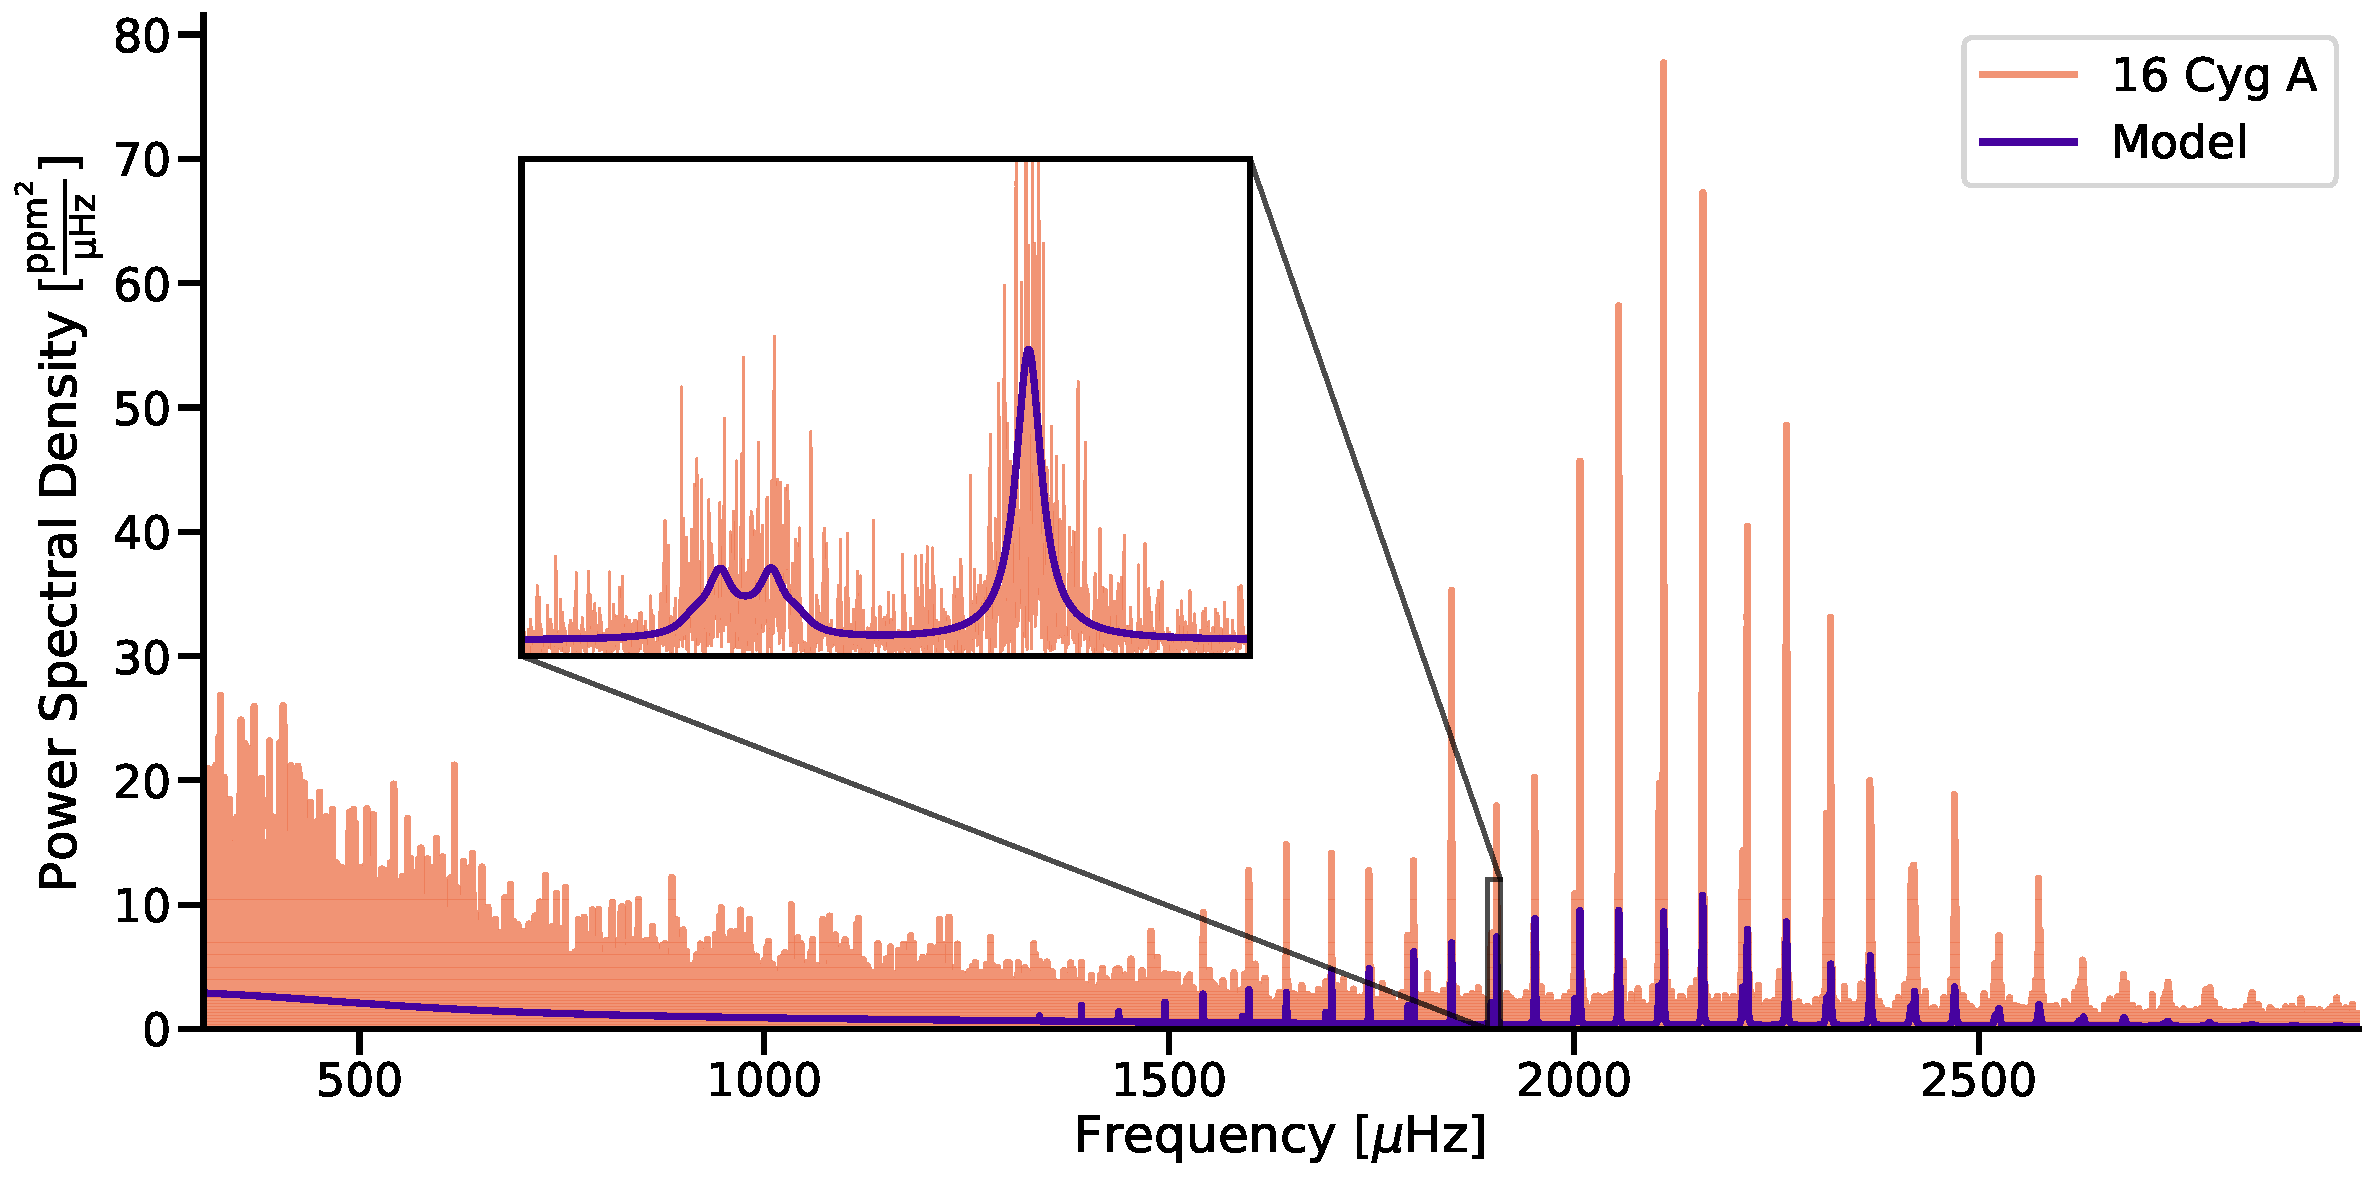
\includegraphics[width=.99\textwidth]{Images/modelfit.pdf}
	\caption{A power spectrum constructed from four years of \kepler observations of 16 Cyg A (KIC 12069424). Plotted over the top is the model resulting from the fit to the data described in this work. The model implements both the mode frequencies, seen on the right hand side of the plot, and the convective background, the effects of which are seen on the left. Low frequencies have been cropped out for clarity. \textit{Inset}: A zoom in on a radial (right) and quadrupole (left) ($\ell = 0, 2$) pair of modes. The quadrupole mode is split into five components by the star's rotation. Due to the star's inclination angle with respect to us, two out of five peaks are more distinct. The height and spacing of the mode components is a function of the star's rotational splitting ($0.56\, \mu\rm{Hz}$, equivalent to $P = 20.5\, \rm{days}$) and angle of inclination ($45^\circ$).}
	\label{fig:modelfit}
\end{figure*}


\section{Verifying asteroseismic results}
\subsection{Priors on rotational parameters}
In our Bayesian analysis, we have placed weakly informative priors on our sampled rotational parameters, $\nu_{\rm s}\sin(i)$ and $\cos(i)$. The prior is especially important for the angle of inclination, which is hardest to infer from the data. We are able to validate the robustness of our asteroseismic results by confirming that their posterior distributions are data-dominated, and not prior-dominated. We can do so by comparing the $68\%$ credible regions of the posterior estimates of $\nu_{\rm s}\sin(i)$ and $i$ against the $68\%$ credible regions of their priors.

A comparison between prior and posterior is shown for 94 stars in $\nu_{\rm s}\sin(i)$, $i$ and $P$ in Supplementary Figure \ref{fig:priors}, arranged by age. In the Figure, results with means (symbols) and $68\%$ credible regions (error bars) that are close to those same values for the prior distribution (where the horizontal line is the mean, and the shaded area is the credible region) can be interpreted as prior-dominated (i.e. poorly informed by the data). Cases where the means differ or the credible regions are smaller than the prior distribution are data-dominated. The projected splitting, $\nu_{\rm s}\sin(i)$, is overall well constrained, with only one star being prior dominated. This is expected, as the projected splitting is what we observe on the star before decoupling inclination and rotation. The angle of inclination $i$, sampled as $\cos(i)$, more closely follows the prior distribution in most cases. Combining the two, the rotation period $P$ has no stars directly corresponding to the effective prior on period, and globally follows a trend with increasing age. The three outliers with fast rotation at late ages (KICs 6603624, 8760414 and 8938364) are discussed in more detail in below.

The rotation rates as presented in this work are a product of our Bayesian sampling of both projected splitting and angle of inclination. As seen in the Figure there are instances where $i$ or $\nu_{\rm s}\sin(i)$ closely resemble the prior (and are therefore prior-dominated). There are no cases of this when looking at the resulting period measurements, as they will have been informed by at least one strongly data-driven parameter (commonly $\nu_{\rm s}\sin(i)$). From this, we concluded that our ensemble of asteroseismic rotation is not strongly dominated by the priors imposed on projected splitting and inclination in our Bayesian analysis.

\begin{figure}
	\centering
	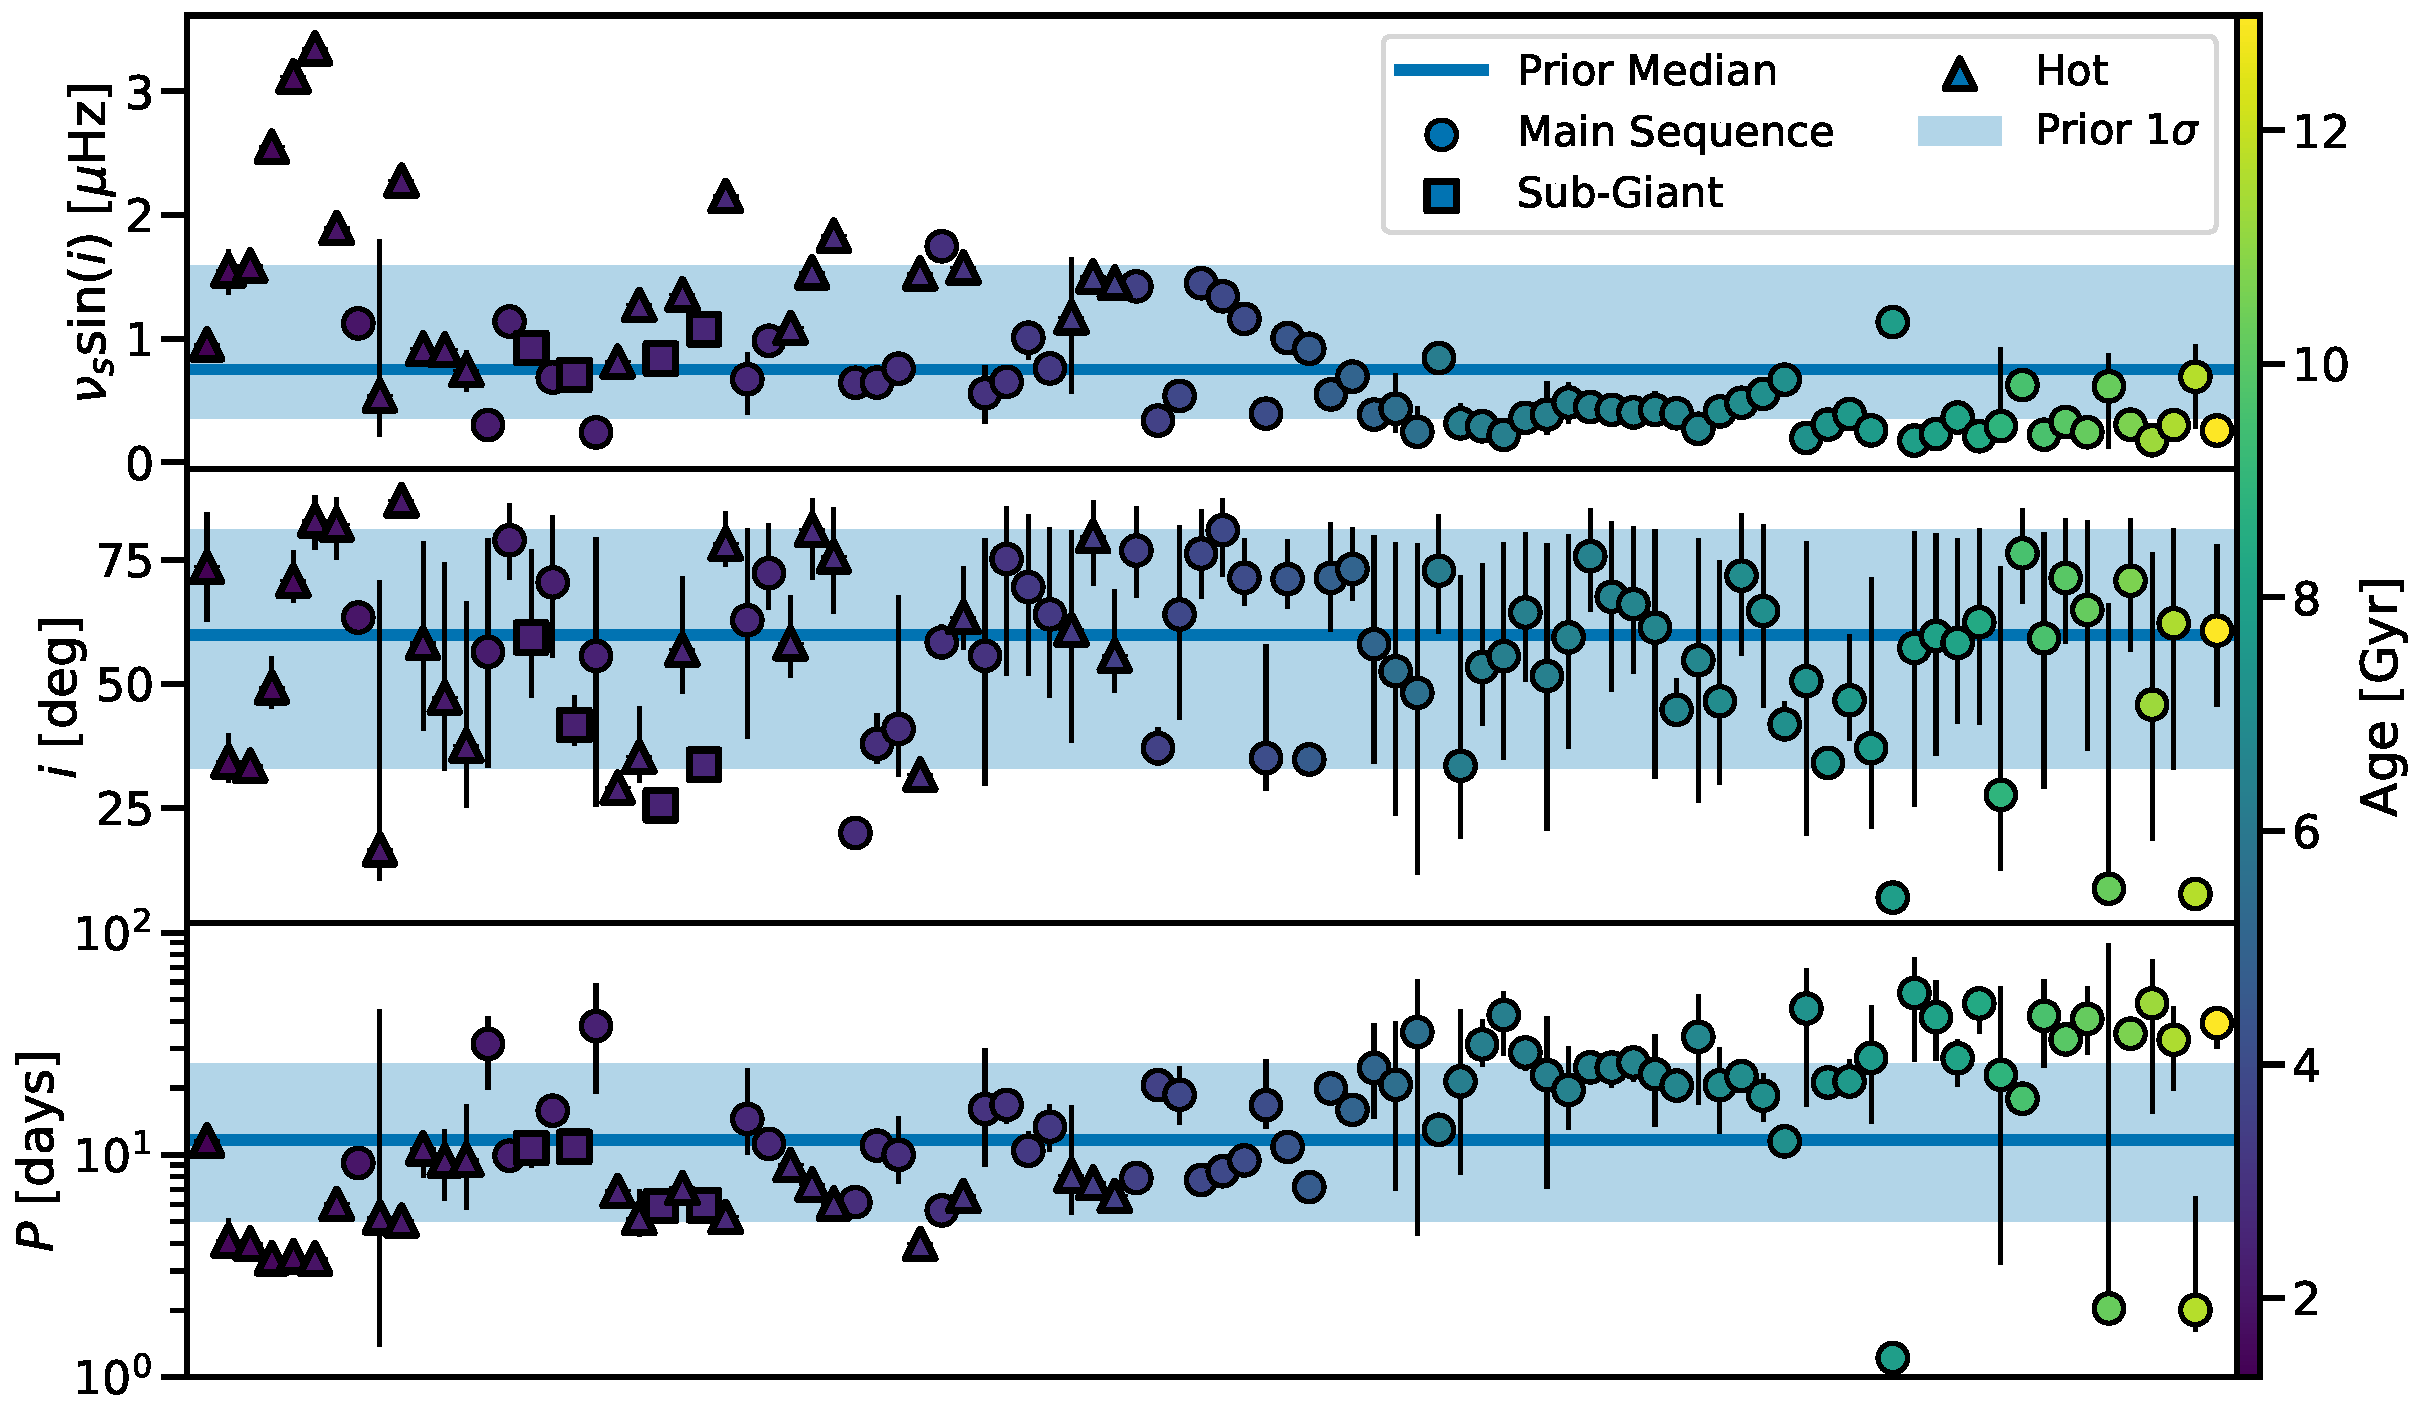
\includegraphics[width=\textwidth]{Images/priors.pdf}
	\caption{\textbf{Comparisons between posterior estimates of rotational parameters (data points and error bars) and the priors on these parameters (shaded regions).} The data are sorted from young stars (left) to old (right). Shown are projected splitting ($\nu_{\rm s}\sin(i)$), inclination angle ($i$, sampled as $\cos(i)$) and rotation period ($P$). Both the prior and values for $P$ are a transformation of the upper two parameters (see text). In all cases, the extent of the error bars and shaded regions indicate the 68\% credible interval of the posterior and prior distributions respectively. The solid lines indicate the median of the prior distributions. In this figure, results with means and errorbars that closely resemble the prior distribution can be interpreted as prior-dominated (i.e. poorly informed by the data). All stars are sorted and coloured and sorted by age. In the case of inclination angle $i$ and rotation period $P$, the displayed priors are transformed from the priors imposed on the sampled parameters from which their posteriors were derived.}
	\label{fig:priors}
\end{figure}

\subsection{Comparisons to previous studies}\label{ssec:litcomp}
In order to validate our results, we compared our rotational parameters to those obtained in the literature, as well as those resulting from the work presented in LEGACY and `Kages', which were unreported and received through private communication by the authors of the catalogue papers.

Comparisons with LEGACY and `Kages' are shown in Supplementary Figure \ref{fig:legacykages} for projected splitting, inclination angle, and rotation period. In all three cases we show the fractional difference between the values obtained in this work and those from LEGACY and `Kages'. On the right of the Figure, we show the distribution of the fractional differences for the three parameters.
The projected splitting is in good agreement with both studies, however LEGACY finds slightly lower $\nu_{\rm s}\sin(i)$ for the faster rotators, deviating from our work by over $1\sigma$. Neither LEGACY nor `Kages' used a spatially isotropic prior for the inclination angle in their analyses, instead opting for a uniform prior. As posterior estimates of inclination angle are only loosely data-driven, the introduction of an isotropic prior should result in our analysis reporting globally higher inclination angles. This effect is seen in the comparisons of both inclination angles and rotation rates for the LEGACY stars, where we find overall lower rotation rates compared to LEGACY for stars at very similar $\nu_{\rm s}\sin(i)$.

A number of stars are excluded from Supplementary Figure \ref{fig:legacykages} and compared individually as extreme outliers: KICs 5094751, 6196457, 8349582, 8494142, 8554498, 105114430 and 11133306 all have fast rotation rates ($<5\, \rm days$) in `Kages', but are found to have a broader spread of rotation rates in this work. At similar values for $\nu_{\rm s}\sin(i)$, `Kages' found much lower inclination angles with highly asymmetrical uncertainties. Based on a comparison between the summary statistics of these stars, we concluded that the results found in this work have better marginalised over inclination angle, improving our measure of rotation.

Conversely, KICs 6603624, 8760414 and 8938364 have extremely slow rotation periods in LEGACY, but extremely \textit{fast} ($<3\, \rm {days}$) in this work. KICs 8760414 and 8938364 are excluded from the gyrochronology analysis below based on checks for $\hat{R}$ and the number of effective samples. Both stars have ages greater than $10\, \rm Gyr$, making their fast rotation rates highly unlikely under any model of rotational evolution. The posterior estimate of $P$ for KIC 6603624 is well-defined in our analysis, but with an age of $7.8\, \rm Gyr$, its measured rotation of $1.2\, \rm days$ is also highly unlikely under any model of rotational evolution. The LEGACY estimate of rotation is similarly extreme at $378\, \rm days$. These three stars have the lowest inclination angles in our sample ($< 10^\circ$), at which point the power in the split components of the seismic modes is so low that it becomes difficult to probe the measure of splitting. The split components for these stars will have a height roughly 3\% of the central mode. For comparison, for the next lowest inclined star at $17^\circ$, this rises to $10\%$. In cases such as these with lower signal-to-noise, spurious peaks may be interpreted as split components.\\

\begin{figure}[h!]
	\centering
	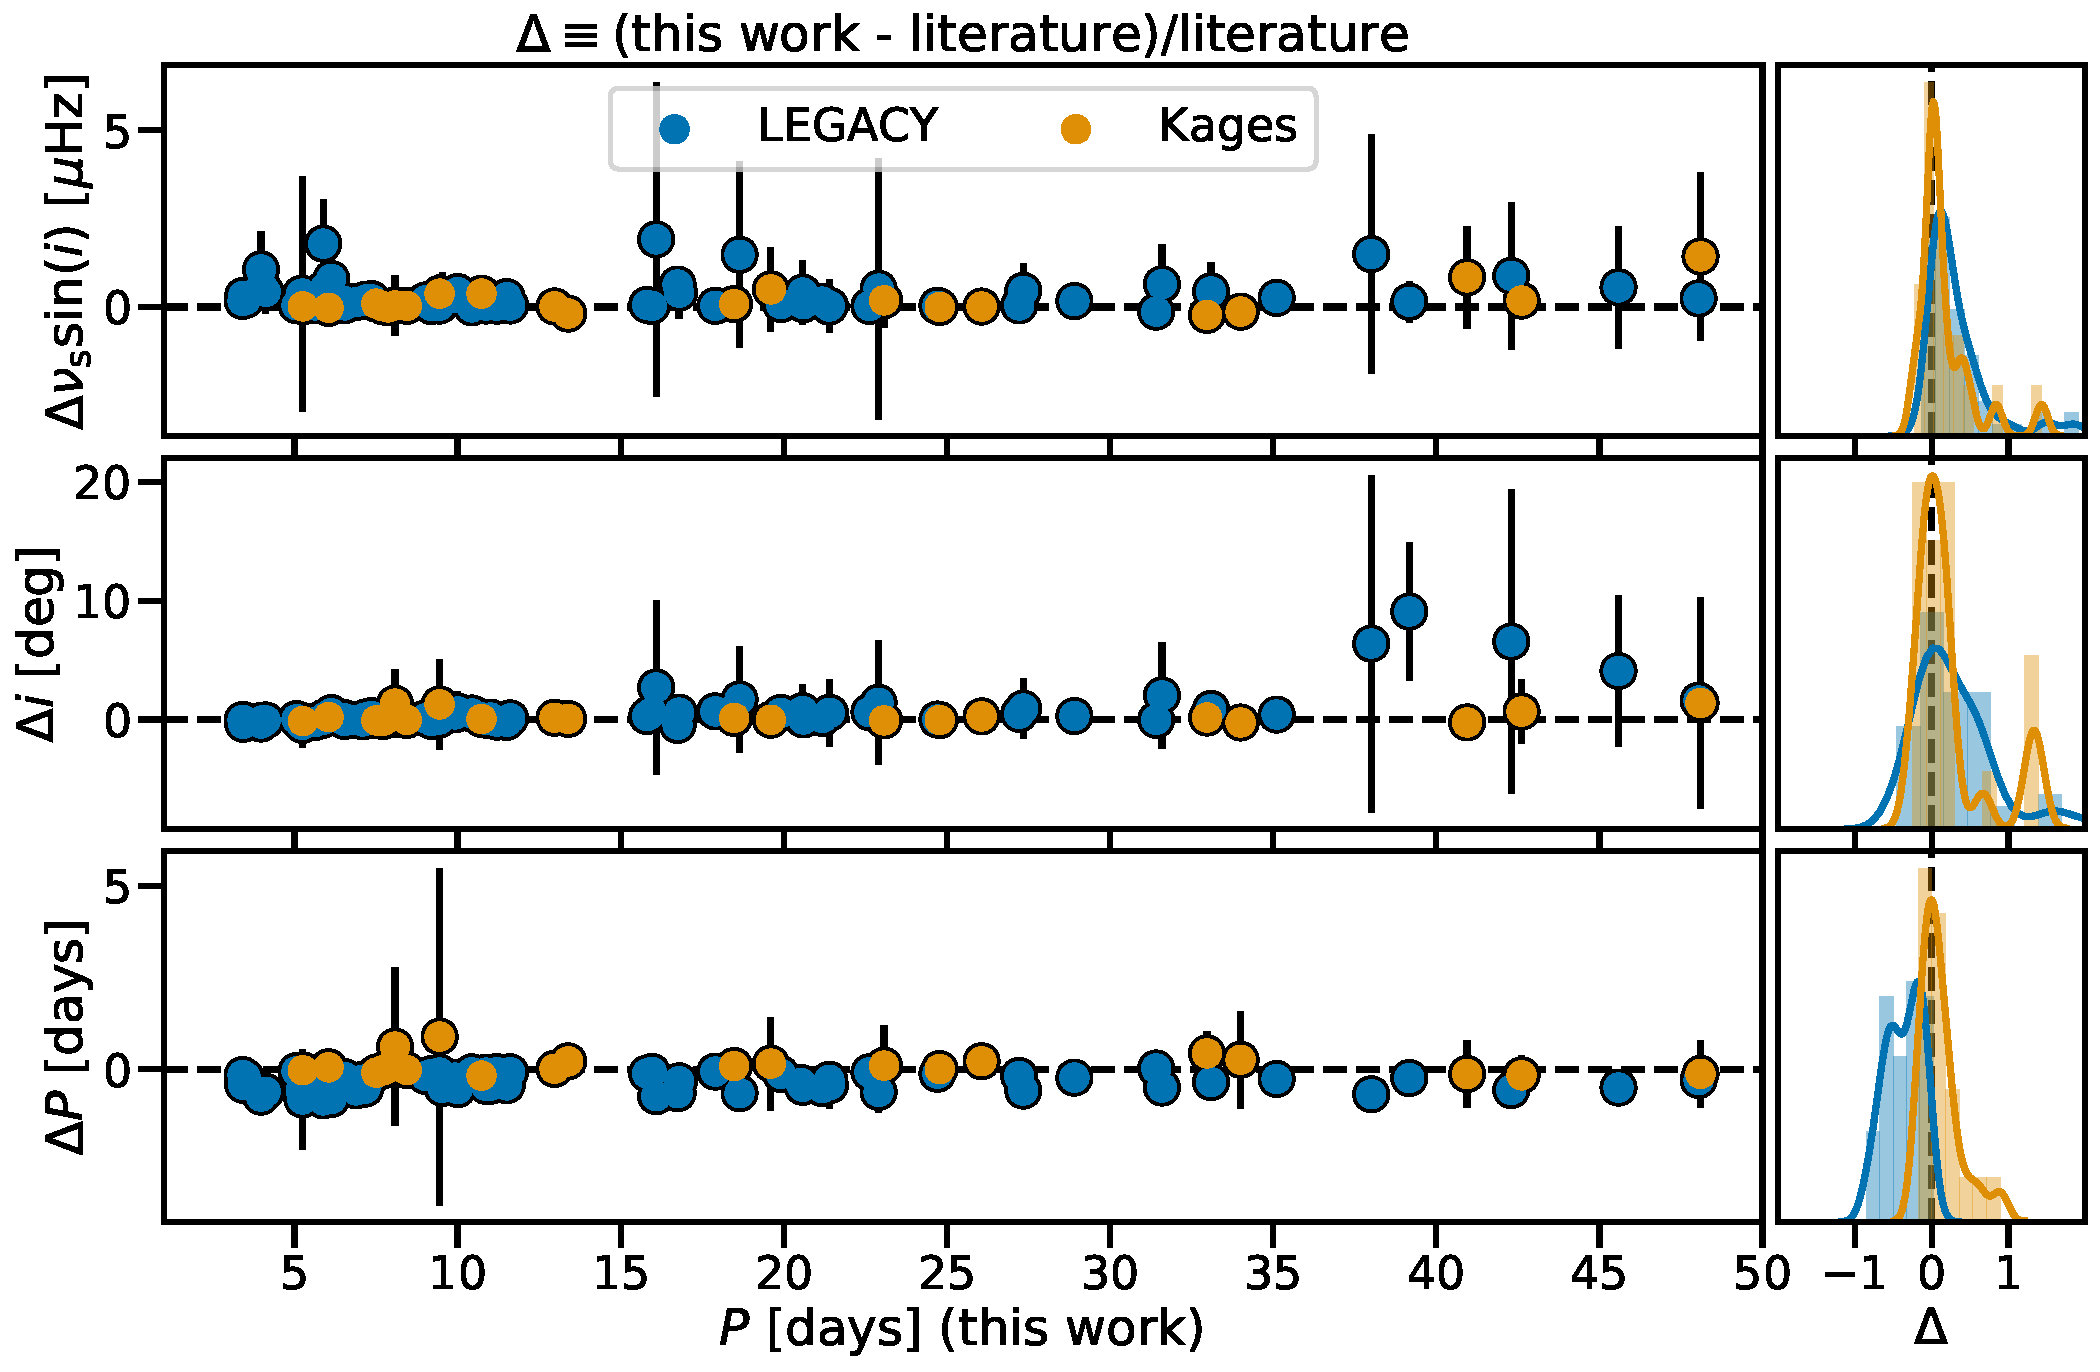
\includegraphics[width=\textwidth]{Images/litcomp_alt2.pdf}
	\caption{\textbf{Comparisons between posterior estimates of rotational parameters from this work and the literature}. Literature values are taken from LEGACY and `Kages' \cite[private communication]{davies+2016, lund+2017}. Shown are projected splitting ($\nu_{\rm s}\sin(i)$), inclination angle ($i$, sampled as $\cos(i)$) and rotation period ($P$). Fractional differences are plotted against stellar rotation obtained in this work. The $\Delta$ indicates the fractional difference between this work and the literature (i.e. stars above the zero-line have higher values in this work). The right hand panels the distribution of the fractional differences around the zero line. The colour legend is consistent throughout all panels. The x-axis units on the right hand panels are equivalent to the y-axis of the left hand panels. 10 stars have been omitted from this plot and are discussed in more detail in the text: KICs 5094751, 6196457, 8349582, 8494142, 8554498, 105114430 and 11133306 all have extremely low rotation periods in Kages, with high uncertainties. Conversely, KICs 6603624, 8760414 and 8938364 have extremely high rotation periods in LEGACY with low uncertainties. Error bars represent the 68\% confidence intervals. In cases where stars had asymmetric error bars, the larger of the two was used when propagating uncertainty for the purposes of this figure.}
	\label{fig:legacykages}
\end{figure}

We also compared our asteroseismic estimates of stellar rotation with similar studies in the literature, shown in Supplementary Figure \ref{fig:literaturecomp}. These included: a study of the binary solar analogues 16 Cyg A \& B \cite{davies+2015}, ; a study of surface and seismic rotation which our catalogue shares 5 stars with \cite{nielsen+2015}, ; and an asteroseismic study of differential rotation with which our catalogue shares 40 targets \cite{benomar+2018}. For the latter, we used their reported splitting value $a_1$, which is equivalent to $\nu_{\rm s}$. 

Overall,  Supplementary Figure \ref{fig:literaturecomp} shows no strong disagreements between our asteroseismic measurements for stellar rotation and those from the literature. The scatter of the fractional differences lies cleanly around the zero line, with a mean and spread of $0.0_{-15.6}^{+16.4}\, \%$. The increase in uncertainty with period is due to more slowly rotating stars being more difficult to constrain using asteroseismology.

It is of note that 16 Cyg A was found to be rotating slightly faster in our analysis compared to the literature \cite{davies+2015} (deviating within $2\sigma$), despite the fit being performed on the same data. We found an inclination angle that is slightly lower for 16 Cyg A but at a similar projected splitting, which would explain finding a lower value of rotation.

There are three outliers at low period in  Supplementary Figure \ref{fig:literaturecomp}: KICs 6603624, 8760414 and 8938364. These are the same targets found to be outliers in a comparison to the LEGACY and `Kages' measurements (see above), with anomalously fast rotation rates and low inclination angles. As these stars represent the lowest inclination angles in our sample, and were found to disagree with two independent studies, we opted to exclude them from the gyrochronology analysis, and to flag the rotation measurements for these three stars presented in this work.


\begin{figure}[h!]
	\centering
	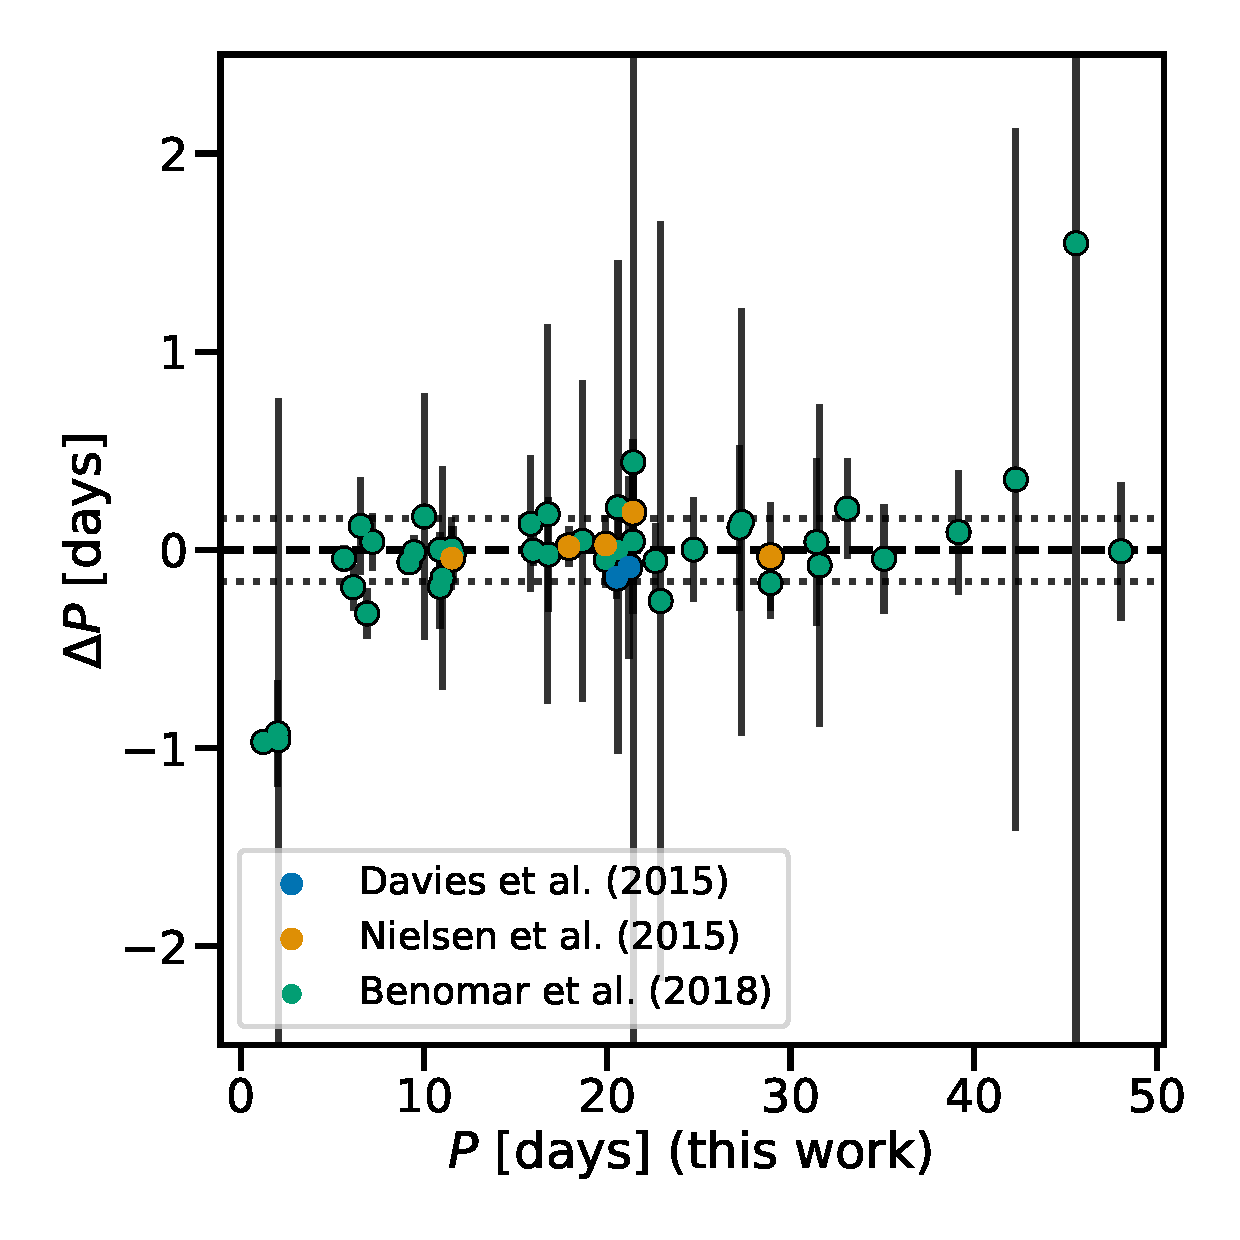
\includegraphics[width=0.8\textwidth]{Images/seis_comparison_rot_alt2.pdf}
	\caption{\textbf{Fractional differences between posterior estimates of asteroseismic rotation period from this work.} Literature sources are: Davies et al. (2015) \cite{davies+2015} (16 Cyg A \& B), Nielsen et al. (2015) \cite{nielsen+2015} (5 stars) and Benomar et al. (2018) \cite{benomar+2018} (40 stars). We used the reported parameter $a_{1}$ from the latter, which represents the rotational splitting in the case of uniform latitudinal rotation in their model. The dashed line represents the median of the sample shown, with the dotted lines representing the $15.9^{\rm{th}}$ and $84.1^{\rm{st}}$ percentiles. Error bars represent the 68\% confidence intervals. In cases where stars had asymmetric error bars, the larger of the two was used when propagating uncertainty for the purposes of this figure.}
	\label{fig:literaturecomp}
\end{figure}

\subsection{Seismic vs spectroscopic rotation}
A distinct difference between rotation rates obtained through different techniques may hold information about differential rotation (both latitudinal and radial) of near-surface layers, such as those we observe in the Sun \cite{beck2000}.  A previous comparison of spectroscopic and seismic rotation rates, performed on a sample of 22 stars, found no significant radial differential rotation \cite{benomar+2018}. In this work they not only considered rotation rates from spots, but also spectroscopic measures of the projected surface rotation $\textrm{v}\sin(i)$, which they found to be more reliable.

With our expanded sample of asteroseismic rotation we can perform a similar analysis, to both validate our sample and probe radial differential rotation.  Supplementary Figure \ref{fig:vsinilit} shows a comparison between spectroscopic $\textrm{v}\sin(i)$ measurements as listed in LEGACY and `Kages' (left) and Benomar et al. (2015) \cite{benomar+2015} (right). In these cases the asteroseismic $\textrm{v}\sin(i)$ has been calculated using our measure of asteroseismic $\nu_s\sin(i)$ and the known asteroseismic radii. Three stars (KICs 6603624, 8760414 and 8938364) have been excluded from this figure due to strong disagreements of measured rotation rates with the literature (see above).

For the LEGACY and `Kages' sample, we find no strong deviation from the 1:1 line except at very low velocities, which is likely due to biases inherent to spectroscopic line broadening measurements \cite{doyle+2014, tayar+2015}. For the Benomar et al. (2015) sample stars lie a lot closer to the 1:1 line.

Overall, there appears to be a global offset where spectroscopic measurements of projected rotation appear faster than asteroseismic measures. Based on the LEGACY and `Kages' $v\sin(i)$ values, this offset is roughly $18\%$ (i.e. spectroscopic projected rotation rates are faster than asteroseismic rates). This offset is much smaller ($\sim5\%$) for the \cite{benomar+2015} sample, albeit for far fewer stars. These offsets are within the typical disagreement between spectroscopic methods, based on comparisons of projected rotation measurements for red giant stars \cite[see Figure 2]{tayar+2015}, especially at $< 5\, \rm{km\,s^{-1}}$.

It is worth addressing the impact this comparison would have on our conclusions for gyrochronology, were we to take the spectroscopic rotation rates as if they were the truth, even at velocities of $< 5\, \rm{km\,s^{-1}}$. For the majority of cases, the seismic velocities are slower than the spectroscopic velocities, which would bias our ensemble towards favouring a standard evolution over a weakened magnetic braking scenario (as stars would overall appear to be rotating slower at late ages). Based on the comparison to spot rotation presented in the main body of this paper, and given known issues comparing seismic and spectroscopic rotation at low velocities, we concluded that the divergence seen in  Supplementary Figure \ref{fig:vsinilit} does not undermine our results.


\begin{figure}[h!]
	\centering
	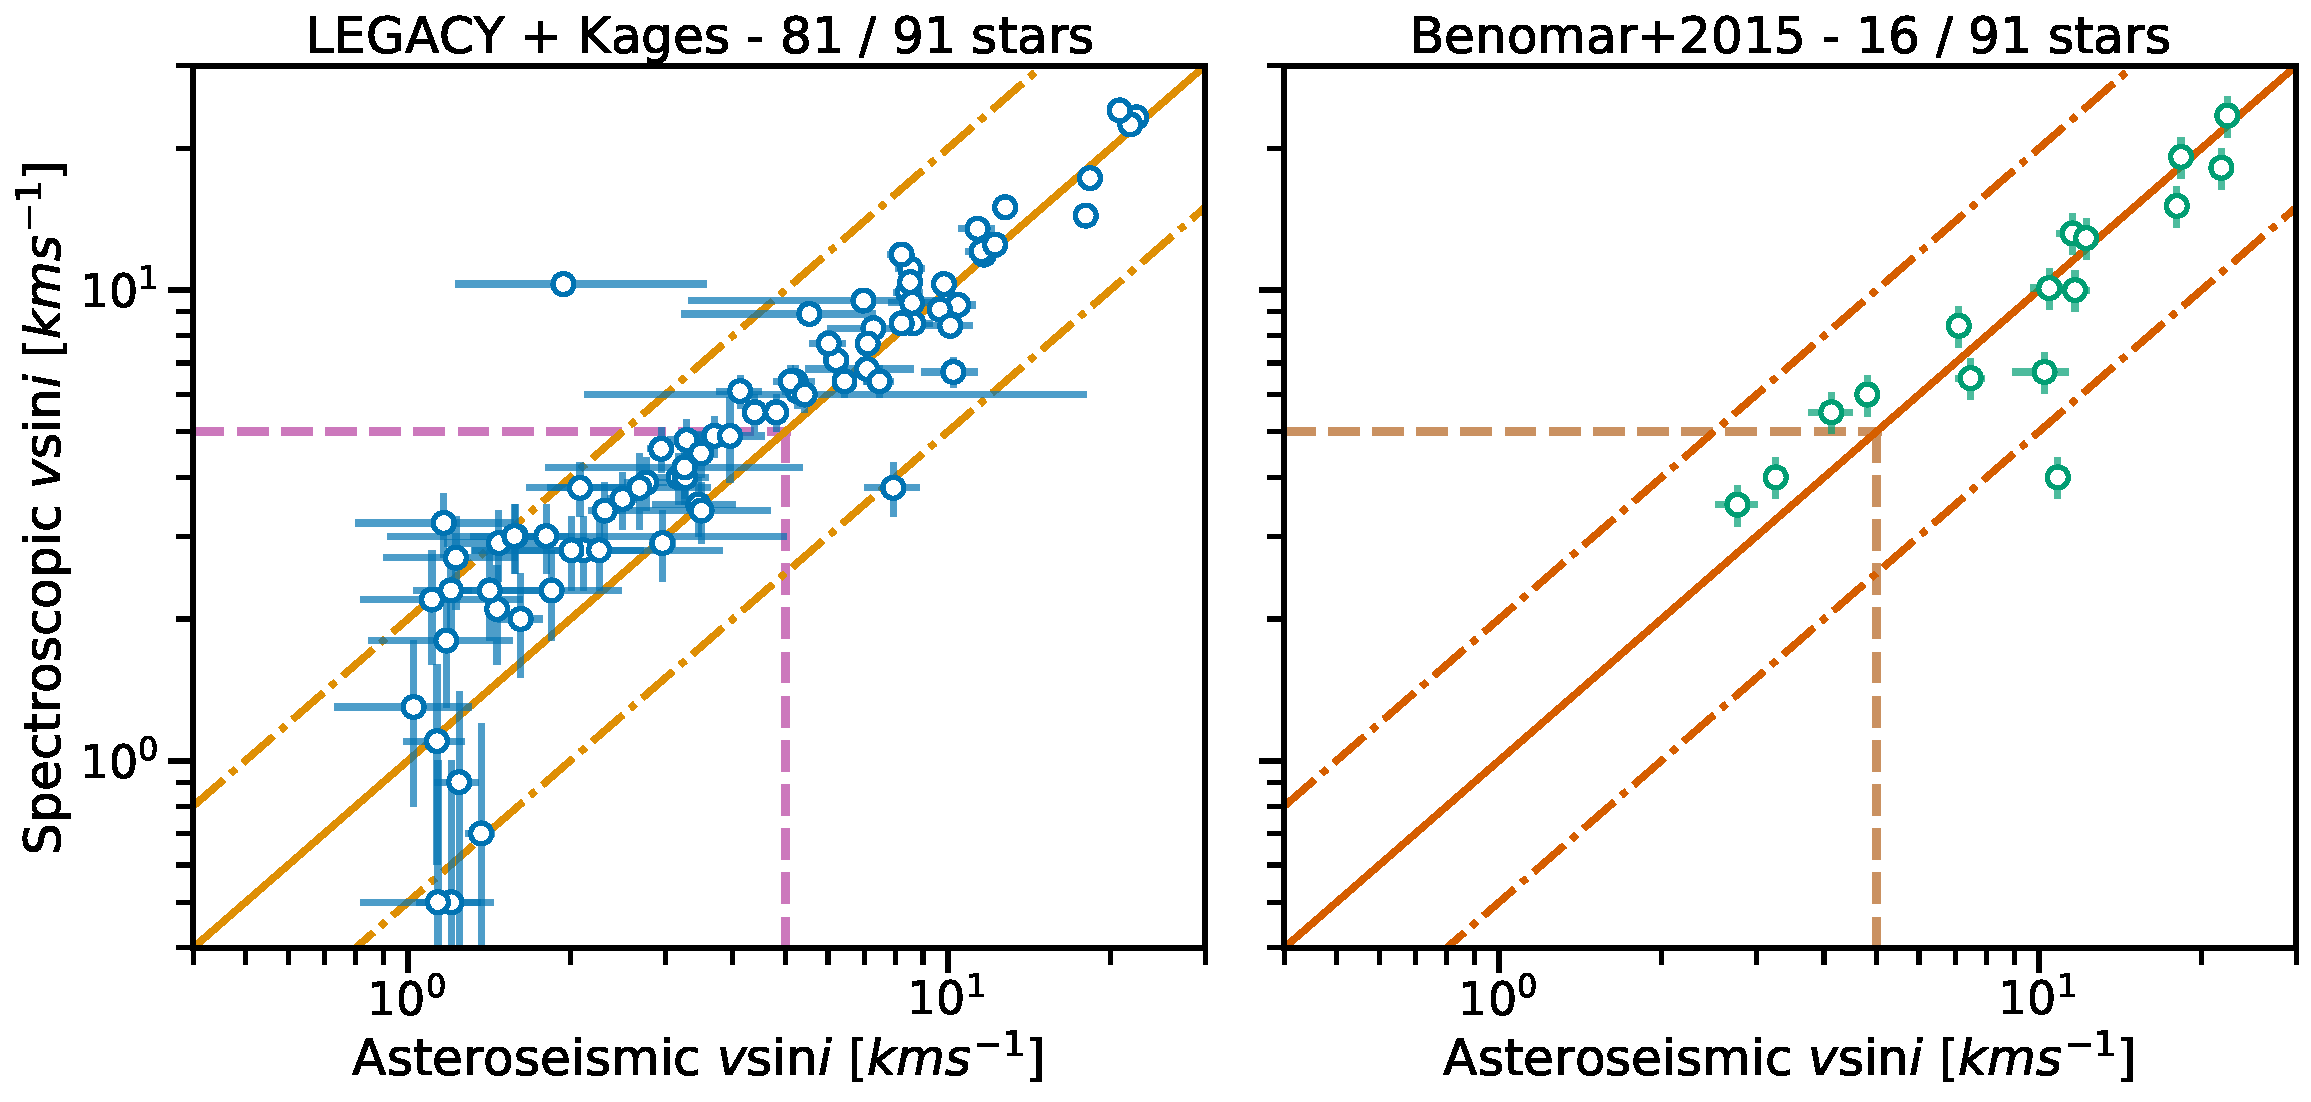
\includegraphics[width=\textwidth]{Images/vsini_comparison_new.pdf}
	\caption{\textbf{Comparisons between asteroseismic and spectroscopic measures of projected surface rotation, $\textrm{v}\sin(i)$.} All asteroseismic (x-axis) values are from this work, all spectroscopic (y-axis) values are from the literature. \textit{Left}: comparisons to 81 stars values reported in LEGACY and Kages. \textit{Right}: comparisons to 16 stars observed by Benomar et al. (2015) \cite{benomar+2015}. Asteroseismic values are transformed from projected splitting ($\nu_s\sin(i)$) using the asteroseismic radius measurements presented in LEGACY and `Kages'. Horizontal error bars represent the 68\% confidence intervals. Vertical error bars represent the formal uncertainty on the published spectroscopic values. The solid lines indicate the 1:1 line, while the dash-dotted lines represent the 2:1 and 1:2 lines. The dashed lines indicate the location of $\textrm{v}\sin(i) = 5\, \rm{kms^{-1}}$, the point at which surface and seismic measures of projected rotation begin to differ strongly \cite{tayar+2015}.}
	\label{fig:vsinilit}
\end{figure}


\subsection{Asteroseismic detection biases}

Stars that are rotating very slowly will show small rotational splittings, which may be indistinguishable from a non-rotating case, wheras stars that are spinning very fast may find that their splitting is so wide that they cross over with split modes at different radial orders ($n$). Asteroseismic selection techniques may also introduce additional biases on a population level. We consider the limitations this places on our asteroseismic method.

\begin{itemize}
	\item \textit{Fast rotating stars:} In prinicple, a star could rotate fast enough that the highest-frequency peak in a split dipole ($\ell = 2$) mode would overlap with the radial ($\ell = 0$) mode. This would occur if $2\nu_{\rm s} > \delta\nu_{02}$, the small separation. For the star in our sample with the smallest $\delta\nu_{02}$ (so the highest risk of this happening), this would occur at a rotation of 8.8 days or faster. For the star with the largest $\delta\nu_{02}$, this limit was roughly 2 days.
	
	In practice, the model still properly fits a spectrum where this kind of mode-overlapping occurs, as the $\ell = 0$ modes don't split, meaning that there are no degenerate solutions in this regime, and further constraints can be obtained from the other modes and split components in the spectrum. A more serious issue may be when the $\ell = 1$ mode at lower frequencies overlaps with the $\ell = 2$ mode as well, which would only occur at a rotation rate of 2 days or faster for the star with the smallest $\delta\nu_{01}$.
	
	\item \textit{Slow rotating stars:} Except for the most rapidly rotating cases, asteroseismic mode splitting is detected by a change in the distribution of the power of mode frequencies as the split components begin to separate from the central mode. If there is to be hard limit at which this measurement is not possible, it should be in the case that $\nu_{\rm s} < 2/T$, where $T$ is the observation time, and $1/T$ is the frequency bin width. For the star in our sample with the shortest observing time, this limit would be $\sim 89$ days, which quickly rises for longer observing baselines. While this constitutes a hard limit, slower rotation rates will become harder and harder to constrain as the rate of splitting becomes smaller. A benefit of the Bayesian approach used in this paper is that it should accurately reflect the increased uncertainty associated with the small rotational splitting.
\end{itemize}

While these two limits cause concern when studying the most extreme rotators, the results presented in this work are driven by stars with rotation rates in the regime of 5 to 30 days. Above, we demonstrated that results on period for these stars were data-driven (i.e. do not reflect the priors), indicating that the splitting is well resolved in this regime, and so we do not expect these limits to bias our conclusions.

Finally, we also consider bias in asteroseismic detections. The probability of an asteroseismic detection with \kepler scales with temperature and radius (i.e. scales inversely with \logg, and therefore main sequence age), and detections are unlikely below roughly $5200\, K$ \cite{chaplin+2011, schofield+2019}. Very young ($\lesssim 2\, \rm{Gyr}$), very magnetically active stars may also suppress their oscillation modes. \cite{mathur+2019}. Though these two effects impose a bias on asteroseismic populations, they do so outside the parameter range on which our comparison takes place. As it is older stars, undergoing magnetic braking, that are required to drive the distinction between stellar models, we conclude that our seismic sample can be assumed to be complete for the purposes of this work.

\section{Verifying consequences for gyrochronology}
\subsection{Limits of our stellar models}\label{ssec:limits}
The rotational stellar models used in this work \cite{vansaders+2019} are constructed for metallicities of $-0.4 < \rm{[Fe/H]} < 0.4\, \rm{dex}$, in steps of $0.1\, \rm {dex}$. Our sample of 91 stars contained 4 stars with metallicities below $-0.4\, \rm{dex}$, which are shown as shaded symbols in Figure 3 in the main paper. Of these, 3 were included in our final sample of 73 stars used to evaluate our stellar models: KICs 7970740, 8684723 and KIC 9965715. All three are classed as MS stars, with metallicities of $-0.54 \pm 0.10$, $-0.42 \pm 0.10$ and $-0.44 \pm 0.18\, \rm {dex}$ respectively, placing them within $3\sigma$ of the metallicity limits of our stellar models. KICs 8684723 and 9965715 strongly agree with the WMB model, whereas KIC 7970740 weakly prefers the standard model. Excluding these stars was not found to significantly alter the joint posterior distribution shown in Figure 4 of the main paper.

A recent study \cite{amard+matt2020} compared different rotational evolution models \cite[of which we use the former in this work]{vansaders+pinsonneault2013, matt+2015} while studying the effect metallicity has on rotation. They found that metal-rich stars spin down significantly more effectively than metal poor stars. The population of 73 stars used in our stellar model comparisons is roughly centered on a $\rm{[Fe/H]}$ of 0 $\rm dex$, with a spread of $~0.16\, \rm dex$, with no stars significantly above or below $\pm 0.4\, \rm dex$ (as discussed above). While differences in stellar rotational evolution as a function of metallicity in this region are still somewhat pronounced, they are much less so than for more metal-rich or poor stars \cite[see Figure 2]{amard+matt2020}. However, for stars with $\feh < 0$, the alternative model prescription \cite{matt+2015} sees stars spin down more slowly than the models used in this work (i.e. they will rotate faster at later ages). This work only explores the presence of weakened magnetic braking for a single braking law, and a comparison to alternative braking model will be explored in a future paper.

When constructing KDEs from our stellar model samples, we selected fixed resolutions (or band-widths) for the KDEs. In mass, the band-width of $0.02\, M_\odot$, was larger than the uncertainties of 24 of 73 stars used to construct our joint posterior. For the stars with the smallest uncertainties, this significantly limits the size of the KDE being evaluated (as subsections of the full stellar models are used to evaluate individual stars, for computational efficiency). In order to confirm that these stars do not significantly affect the ensemble's preference towards the WMB model, we recalculated the joint posterior distribution for $Q_{\rm WMB}$, excluding stars with an uncertainty on mass smaller than the KDE band-width. While the 24 stars with small uncertainties do favour the WMB model, they do so very weakly, whereas the remaining 49 stars with larger uncertainties strongly favour the WMB model. Their removal from the total joint posterior probability does not significantly alter it from the distribution shown in Figure 4 of the main paper.

\subsection{Systematic uncertainties from asteroseismology}
In our model analysis, we used asteroseismic mass and age obtained using \texttt{BASTA}, as reported in LEGACY and Kages. Asteroseismic properties obtained through stellar models can be subject to systematic errors arising from differences in input physics and choice of stellar models not included in the reported statistical uncertainties. A quantification of these different systematic effects can be found in the `Kages' catalogue paper \cite{silvaaguirre+2015}. Combining their reported median systematic uncertainties due to input physics results in median uncertainties of $20\%$ (up from $14\%)$ on age and $5\%$ (up from $3\%$) on mass for the `Kages' sample. For LEGACY, the median uncertainties are $18\%$ (up from $10\%)$ and $5.6\%$ (up from $4\%$) for age and mass respectively.

We re-ran our model analysis after inflating uncertainties on mass and age. We increased uncertainties by the fractional difference between the \texttt{BASTA} statistical uncertainties and the median full statistical and systematic uncertainties described above. For example, a LEGACY star with a mass of $2.0 \pm 0.5\, M_\odot$ would have its uncertainty inflated by $1.6\%$ of its mass, to $0.53\, M_\odot$. 

To further test the limits of this analysis, we also reran our mixture model fit, this time only shifting the asteroseismic ages younger by the systematic uncertainty, and retaining the statistical uncertainty (i.e. the ages of LEGACY and `Kages' stars were reduced by $8\%$ and $6\%$ respectively). In this scenario where all asteroseismic ages are overestimated, `true' fast rotators at young ages would have been mistaken for fast rotators at old ages, suggesting the presence of weakened magnetic braking where none existed. 

The results of these tests are discussed further in the main body of the paper.

\subsection{Binaries and Planet Hosts}
For stars to be good probes of existing gyrochronology relations, their rotational evolution must occur in isolation. If a star interacts with a close binary companion (through tides, or a merger) the natural angular momentum loss can be disturbed, causing gyrochronology to mispredict ages \cite{leiner+2019, fleming+2019}. Between LEGACY and Kages, we have 8 known binaries. 

First, KIC 8379927, KIC 7510397, KIC 10454113 and KIC 9025370 are spectroscopic binaries. This does not affect the asteroseismic analysis, but may affect their rotational evolution. Of these, KICs 8379927, 7510397 and 9025370 were included in the gyrochronology analysis. None of them preferred one model strongly over the other, with all three finding flat posteriors for $Q_{\rm WMB}$.

Second, the binary pairs of KIC 9139151 \& 9139163 and 16 Cyg A \& B are individually observed binary components with wide orbital separations, so we do not expect their binarity to have affected their rotational evolution \cite{halbwachs1986, white+2013}. 

While we chose not to account for star-planet tidal interactions in this work, we note that this may disturb the natural stellar rotational evolution when tidal forces are at play \cite{maxted+2015, gallet+delorme2019, benbakoura+2019}, although this has been disputed by observations of asteroseismic planet hosts \cite{ceillier+2016}.\\



\section{Supplementary Table}
\begin{landscape}
\setlength\LTleft{0pt}
\setlength\LTright{0pt}
\footnotesize
\begin{longtable}{c|ccccc|ccc|ccc}
	\caption{Parameters for the 94 stars for which seismic rotation rates were obtained in this work. Temperature (\teff), age, mass, metallicity (\feh) and surface gravity ($\log(g)$) are adopted from the LEGACY \cite[L]{lund+2017,silvaaguirre+2017} and`Kages' \cite[K]{silvaaguirre+2015,davies+2016} catalogues, as listed in the Source column. Projected splitting ($\nu_{\rm s}\sin(i)$), inclination angle ($i$) and asteroseismic rotation ($P$) are from this work. Uncertainties were taken using the $15.9^{\rm th}$ and $84.1^{\rm st}$ percentiles of posterior distributions on the parameters, which are frequently asymmetrical in linear space. Reported values are the median of the posteriors. For parameters with no direct posterior samples (e.g. rotation) the full posterior samples were transformed before taking the summary statistics. The stellar type denotes whether a star is roughly classified as belonging to the main sequence (MS), Sub-Giants (SG) or `hot' stars (H) (see text).
		The flags indicate the following: 0; no issues, used in the gyrochronology analysis. 1; has either a number of effective samples $n_{\rm eff} < 1000$ for the asteroseismic splitting, or Gelman-Rubin convergence metric of $\hat{R} > 1.1$ \cite{gelman+rubin1992}, indicating that rotation measurements for these stars are less robust than those with a flag of 0. 2; was found to strongly disagree with multiple literature values, excluded from the gyrochronology analysis. 3; fell outside the model range of the stellar models, and were therefore not used in the gyrochronology analysis. Table is continued on the next page. A machine-readable version of the table is available (as Supplementary Data 1).}\label{tab:results}\\
	\toprule
	KIC & $T_{\rm{eff}}$ & Age & Mass & \feh & $\log(g)$ & $\nu_{\rm{s}}\sin(i)$ & $i$   & $P$   &  Flag & Type & Source \\
	& [$\mathrm{K}$] &  [$\mathrm{Gyr}$] & [$\mathrm{M_{\odot}}$] & [$\mathrm{dex}$] & [$\mathrm{dex}$] & [$\mathrm{\mu Hz}$]  & [$\mathrm{{}^{\circ}}$] & [$\mathrm{days}$]   &  &  &  \\
	\midrule
	\endfirsthead
	\caption[]{\textit{Continued from previous page.}}\\
	\toprule
	KIC & $T_{\rm{eff}}$ & Age & Mass & \feh & $\log(g)$ & $\nu_{\rm{s}}\sin(i)$ & $i$   & $P$   &  Flag & Type & Source \\
	& [$\mathrm{K}$] &  [$\mathrm{Gyr}$] & [$\mathrm{M_{\odot}}$] & [$\mathrm{dex}$] & [$\mathrm{dex}$] & [$\mathrm{\mu Hz}$]  & [$\mathrm{{}^{\circ}}$] & [$\mathrm{days}$]   &  &  &  \\
	\midrule
	\endhead
	\bottomrule \multicolumn{12}{r}{\textit{Continued on next page}}\\
	\endfoot
	\bottomrule
	\endlastfoot
	
	1435467 & 6326$\pm$77    & 3.02$_{-0.35}^{+0.50}$    & 1.32$_{-0.05}^{+0.03}$ & 0.01$\pm$0.10     & 4.100$_{-0.009}^{+0.009}$ & 1.58$_{-0.09}^{+0.10}$ & 63.4$_{-6.6}^{+10.2}$     & 6.5$_{-0.6}^{+0.8}$      & 0 &        H & L \\
	2837475 & 6614$\pm$77    & 1.63$_{-0.18}^{+0.11}$    & 1.43$_{-0.02}^{+0.02}$ & 0.01$\pm$0.10     & 4.163$_{-0.007}^{+0.007}$ & 3.12$_{-0.08}^{+0.08}$ & 70.7$_{-4.4}^{+6.0}$      & 3.5$_{-0.2}^{+0.2}$      & 0 &        H & L \\
	3425851 & 6343$\pm$85    & 3.32$_{-0.64}^{+0.85}$    & 1.18$_{-0.05}^{+0.05}$ & -0.04$\pm$0.10    & 4.243$_{-0.008}^{+0.008}$ & 1.17$_{-0.62}^{+0.48}$ & 60.9$_{-22.7}^{+20.1}$    & 8.1$_{-2.7}^{+8.6}$      & 0 &        H & K \\
	3427720 & 6045$\pm$77    & 2.23$_{-0.24}^{+0.24}$    & 1.11$_{-0.01}^{+0.02}$ & -0.06$\pm$0.10    & 4.387$_{-0.004}^{+0.005}$ & 0.30$_{-0.06}^{+0.06}$ & 56.4$_{-23.4}^{+22.9}$    & 31.6$_{-11.8}^{+10.2}$   & 0 &        MS & L \\
	3456181 & 6384$\pm$77    & 2.09$_{-0.13}^{+0.13}$    & 1.50$_{-0.02}^{+0.03}$ & -0.15$\pm$0.10    & 3.949$_{-0.009}^{+0.008}$ & 0.92$_{-0.08}^{+0.08}$ & 58.2$_{-17.7}^{+20.4}$    & 10.7$_{-2.8}^{+2.0}$     & 0 &        H & L \\
	3544595 & 5669$\pm$75    & 6.63$_{-0.57}^{+0.62}$    & 0.90$_{-0.01}^{+0.01}$ & -0.18$\pm$0.10    & 4.468$_{-0.003}^{+0.003}$ & 0.40$_{-0.04}^{+0.04}$ & 66.0$_{-13.9}^{+15.6}$    & 26.1$_{-4.7}^{+3.9}$     & 0 &        MS & K \\
	3632418 & 6193$\pm$77    & 2.63$_{-0.18}^{+0.18}$    & 1.41$_{-0.02}^{+0.02}$ & -0.12$\pm$0.10    & 4.024$_{-0.008}^{+0.008}$ & 0.98$_{-0.03}^{+0.03}$ & 72.3$_{-7.4}^{+10.0}$     & 11.2$_{-0.7}^{+0.6}$     & 0 &        MS & L \\
	3656476 & 5668$\pm$77    & 8.37$_{-1.57}^{+1.72}$    & 1.04$_{-0.04}^{+0.05}$ & 0.25$\pm$0.10     & 4.225$_{-0.010}^{+0.008}$ & 0.21$_{-0.02}^{+0.02}$ & 62.4$_{-20.5}^{+18.9}$    & 48.0$_{-12.7}^{+8.1}$    & 0 &        MS & L \\
	3735871 & 6107$\pm$77    & 2.35$_{-0.85}^{+1.04}$    & 1.09$_{-0.04}^{+0.04}$ & -0.04$\pm$0.10    & 4.396$_{-0.007}^{+0.007}$ & 0.69$_{-0.05}^{+0.05}$ & 70.4$_{-15.1}^{+13.4}$    & 15.8$_{-2.5}^{+1.8}$     & 0 &        MS & L \\
	4141376 & 6134$\pm$91    & 3.27$_{-0.64}^{+0.59}$    & 1.02$_{-0.03}^{+0.02}$ & -0.24$\pm$0.10    & 4.412$_{-0.003}^{+0.004}$ & 0.76$_{-0.13}^{+0.13}$ & 64.0$_{-16.7}^{+17.5}$    & 13.4$_{-3.0}^{+3.4}$     & 0 &        MS & K \\
	4143755 & 5622$\pm$106   & 11.27$_{-1.35}^{+1.50}$   & 0.92$_{-0.03}^{+0.02}$ & -0.40$\pm$0.11    & 4.102$_{-0.001}^{+0.002}$ & 0.18$_{-0.05}^{+0.08}$ & 45.8$_{-27.3}^{+30.6}$    & 48.1$_{-32.7}^{+27.4}$   & 1 &        MS & K \\
	4349452 & 6270$\pm$79    & 3.45$_{-0.72}^{+0.81}$    & 1.16$_{-0.05}^{+0.04}$ & -0.04$\pm$0.10    & 4.275$_{-0.007}^{+0.008}$ & 1.50$_{-0.09}^{+0.09}$ & 79.7$_{-10.0}^{+7.1}$      & 7.5$_{-0.6}^{+0.5}$     & 0 &        H & K \\
	4914423 & 5845$\pm$88    & 6.67$_{-0.62}^{+0.69}$    & 1.10$_{-0.03}^{+0.02}$ & 0.07$\pm$0.11     & 4.155$_{-0.004}^{+0.004}$ & 0.42$_{-0.14}^{+0.15}$ & 61.3$_{-30.5}^{+19.8}$    & 23.1$_{-9.6}^{+11.7}$    & 0 &        MS & K \\
	4914923 & 5805$\pm$77    & 7.57$_{-1.79}^{+1.66}$    & 1.06$_{-0.05}^{+0.06}$ & 0.08$\pm$0.10     & 4.197$_{-0.010}^{+0.008}$ & 0.39$_{-0.03}^{+0.03}$ & 46.6$_{-8.1}^{+13.3}$     & 21.4$_{-3.5}^{+5.4}$     & 0 &        MS & L \\
	5094751 & 5952$\pm$75    & 6.35$_{-1.05}^{+1.05}$    & 1.07$_{-0.04}^{+0.04}$ & -0.08$\pm$0.10    & 4.213$_{-0.008}^{+0.007}$ & 0.39$_{-0.16}^{+0.27}$ & 51.5$_{-31.1}^{+26.7}$    & 22.9$_{-15.8}^{+19.3}$   & 0 &        MS & K \\
	5184732 & 5846$\pm$77    & 4.85$_{-0.88}^{+1.57}$    & 1.15$_{-0.06}^{+0.04}$ & 0.36$\pm$0.10     & 4.255$_{-0.008}^{+0.010}$ & 0.55$_{-0.02}^{+0.02}$ & 71.3$_{-10.8}^{+11.2}$    & 19.9$_{-1.9}^{+1.3}$     & 0 &        MS & L \\
	5773345 & 6130$\pm$84    & 2.55$_{-0.24}^{+0.26}$    & 1.47$_{-0.03}^{+0.03}$ & 0.21$\pm$0.09     & 3.993$_{-0.007}^{+0.008}$ & 1.08$_{-0.08}^{+0.08}$ & 33.7$_{-2.5}^{+2.8}$      & 5.9$_{-0.5}^{+0.7}$      & 0 &        SG & L \\
	5866724 & 6169$\pm$50    & 3.89$_{-0.48}^{+0.59}$    & 1.20$_{-0.03}^{+0.03}$ & 0.09$\pm$0.08     & 4.224$_{-0.005}^{+0.007}$ & 1.34$_{-0.08}^{+0.07}$ & 80.9$_{-9.4}^{+6.3}$      & 8.4$_{-0.5}^{+0.5}$      & 0 &        MS & K \\
	5950854 & 5853$\pm$77    & 8.93$_{-1.15}^{+1.12}$    & 0.97$_{-0.03}^{+0.03}$ & -0.23$\pm$0.10    & 4.238$_{-0.007}^{+0.007}$ & 0.29$_{-0.12}^{+0.64}$ & 27.6$_{-15.2}^{+46.0}$    & 22.9$_{-19.7}^{+34.2}$   & 1 &        MS & L \\
	6106415 & 6037$\pm$77    & 5.03$_{-1.12}^{+1.28}$    & 1.07$_{-0.04}^{+0.05}$ & -0.04$\pm$0.10    & 4.295$_{-0.009}^{+0.009}$ & 0.69$_{-0.02}^{+0.02}$ & 73.1$_{-6.3}^{+8.4}$      & 16.0$_{-0.8}^{+0.7}$     & 0 &        MS & L \\
	6116048 & 6033$\pm$77    & 9.58$_{-1.90}^{+2.16}$    & 0.94$_{-0.05}^{+0.05}$ & -0.23$\pm$0.10    & 4.254$_{-0.012}^{+0.009}$ & 0.63$_{-0.02}^{+0.02}$ & 76.3$_{-10.2}^{+9.0}$     & 17.9$_{-1.2}^{+0.8}$     & 0 &        MS & L \\
	6196457 & 5871$\pm$94    & 5.52$_{-0.48}^{+0.51}$    & 1.21$_{-0.03}^{+0.02}$ & 0.17$\pm$0.11     & 4.049$_{-0.004}^{+0.005}$ & 0.43$_{-0.19}^{+0.28}$ & 52.5$_{-29.1}^{+26.0}$    & 20.7$_{-13.7}^{+19.2}$   & 0 &        MS & K \\
	6225718 & 6313$\pm$76    & 2.41$_{-0.43}^{+0.53}$    & 1.16$_{-0.03}^{+0.03}$ & -0.07$\pm$0.10    & 4.319$_{-0.007}^{+0.005}$ & 0.81$_{-0.03}^{+0.03}$ & 29.1$_{-1.8}^{+2.1}$      & 6.9$_{-0.5}^{+0.6}$      & 0 &        H & L \\
	6278762 & 5046$\pm$74    & 11.54$_{-0.94}^{+0.99}$   & 0.74$_{-0.01}^{+0.01}$ & -0.37$\pm$0.09    & 4.560$_{-0.003}^{+0.002}$ & 0.30$_{-0.09}^{+0.09}$ & 62.2$_{-29.5}^{+19.0}$    & 33.0$_{-13.5}^{+13.6}$   & 1, 3 &        MS & K \\
	6508366 & 6331$\pm$77    & 2.06$_{-0.14}^{+0.13}$    & 1.53$_{-0.02}^{+0.03}$ & -0.05$\pm$0.10    & 3.942$_{-0.007}^{+0.005}$ & 2.28$_{-0.04}^{+0.04}$ & 87.0$_{-3.2}^{+2.1}$      & 5.1$_{-0.1}^{+0.1}$      & 0 &        H & L \\
	6521045 & 5825$\pm$75    & 6.50$_{-0.56}^{+0.46}$    & 1.11$_{-0.02}^{+0.02}$ & 0.02$\pm$0.10     & 4.125$_{-0.004}^{+0.004}$ & 0.45$_{-0.02}^{+0.03}$ & 75.7$_{-11.2}^{+9.7}$     & 24.8$_{-2.0}^{+1.9}$     & 0 &        MS & K \\
	6603624 & 5674$\pm$77    & 7.82$_{-0.86}^{+0.94}$    & 1.01$_{-0.02}^{+0.03}$ & 0.28$\pm$0.10     & 4.320$_{-0.005}^{+0.004}$ & 1.13$_{-0.13}^{+0.13}$ & 6.9$_{-0.8}^{+0.8}$       & 1.2$_{-0.0}^{+0.0}$      & 2 &        MS & L \\
	6679371 & 6479$\pm$77    & 1.95$_{-0.16}^{+0.18}$    & 1.53$_{-0.02}^{+0.04}$ & 0.01$\pm$0.10     & 3.934$_{-0.008}^{+0.007}$ & 1.90$_{-0.06}^{+0.05}$ & 82.1$_{-7.2}^{+5.5}$      & 6.0$_{-0.2}^{+0.2}$      & 0 &        H & L \\
	6933899 & 5832$\pm$77    & 6.34$_{-0.62}^{+0.72}$    & 1.13$_{-0.03}^{+0.03}$ & -0.01$\pm$0.10    & 4.087$_{-0.007}^{+0.008}$ & 0.36$_{-0.02}^{+0.02}$ & 64.3$_{-14.0}^{+16.1}$    & 28.9$_{-4.8}^{+3.7}$     & 0 &        MS & L \\
	7103006 & 6344$\pm$77    & 2.47$_{-0.24}^{+0.22}$    & 1.42$_{-0.02}^{+0.04}$ & 0.02$\pm$0.10     & 4.015$_{-0.007}^{+0.007}$ & 1.36$_{-0.09}^{+0.08}$ & 56.8$_{-8.8}^{+14.8}$     & 7.1$_{-1.0}^{+1.3}$      & 0 &        H & L \\
	7106245 & 6068$\pm$102   & 6.27$_{-1.06}^{+1.06}$    & 0.92$_{-0.04}^{+0.02}$ & -0.99$\pm$0.19    & 4.325$_{-0.007}^{+0.007}$ & 0.32$_{-0.10}^{+0.16}$ & 33.4$_{-14.7}^{+38.4}$    & 21.4$_{-13.2}^{+23.8}$   & 1, 3 &        MS & L \\
	7206837 & 6305$\pm$77    & 2.90$_{-0.30}^{+0.42}$    & 1.30$_{-0.03}^{+0.03}$ & 0.10$\pm$0.10     & 4.163$_{-0.007}^{+0.008}$ & 1.53$_{-0.12}^{+0.12}$ & 31.7$_{-2.8}^{+3.2}$      & 4.0$_{-0.4}^{+0.6}$      & 0 &        H & L \\
	7296438 & 5775$\pm$77    & 7.23$_{-1.77}^{+1.49}$    & 1.08$_{-0.05}^{+0.06}$ & 0.19$\pm$0.10     & 4.201$_{-0.010}^{+0.009}$ & 0.20$_{-0.06}^{+0.06}$ & 50.5$_{-31.1}^{+28.2}$    & 45.6$_{-29.0}^{+23.4}$   & 1 &        MS & L \\
	7510397 & 6171$\pm$77    & 2.82$_{-0.16}^{+0.14}$    & 1.37$_{-0.02}^{+0.02}$ & -0.21$\pm$0.10    & 4.036$_{-0.004}^{+0.007}$ & 0.64$_{-0.06}^{+0.06}$ & 19.9$_{-2.0}^{+2.0}$      & 6.1$_{-0.6}^{+0.7}$      & 0 &        MS & L \\
	7670943 & 6463$\pm$110   & 2.78$_{-0.51}^{+0.62}$    & 1.24$_{-0.05}^{+0.04}$ & 0.09$\pm$0.11     & 4.228$_{-0.008}^{+0.008}$ & 1.83$_{-0.14}^{+0.14}$ & 75.7$_{-11.5}^{+9.8}$     & 6.0$_{-0.6}^{+0.6}$      & 0 &        H & K \\
	7680114 & 5811$\pm$77    & 7.68$_{-1.28}^{+1.45}$    & 1.06$_{-0.05}^{+0.04}$ & 0.05$\pm$0.10     & 4.172$_{-0.010}^{+0.008}$ & 0.26$_{-0.04}^{+0.05}$ & 37.0$_{-16.3}^{+34.3}$    & 27.3$_{-13.5}^{+19.6}$   & 0 &        MS & L \\
	7771282 & 6248$\pm$77    & 3.24$_{-0.32}^{+0.35}$    & 1.29$_{-0.03}^{+0.03}$ & -0.02$\pm$0.10    & 4.112$_{-0.007}^{+0.007}$ & 1.01$_{-0.18}^{+0.14}$ & 69.5$_{-17.8}^{+14.6}$    & 10.4$_{-1.7}^{+2.3}$     & 0 &        MS & L \\
	7871531 & 5501$\pm$77    & 9.96$_{-1.77}^{+1.93}$    & 0.83$_{-0.02}^{+0.03}$ & -0.26$\pm$0.10    & 4.478$_{-0.005}^{+0.007}$ & 0.33$_{-0.03}^{+0.03}$ & 71.3$_{-13.2}^{+12.0}$    & 33.1$_{-4.1}^{+4.1}$     & 0 &        MS & L \\
	7940546 & 6235$\pm$77    & 2.33$_{-0.08}^{+0.08}$    & 1.40$_{-0.01}^{+0.03}$ & -0.20$\pm$0.10    & 4.007$_{-0.001}^{+0.003}$ & 1.14$_{-0.03}^{+0.03}$ & 78.9$_{-7.9}^{+7.4}$      & 9.9$_{-0.4}^{+0.3}$      & 0 &        MS & L \\
	7970740 & 5309$\pm$77    & 12.98$_{-2.00}^{+1.36}$   & 0.73$_{-0.01}^{+0.03}$ & -0.54$\pm$0.10    & 4.539$_{-0.005}^{+0.004}$ & 0.26$_{-0.02}^{+0.03}$ & 60.7$_{-15.3}^{+17.4}$    & 39.2$_{-9.0}^{+6.7}$     & 0 &        MS & L \\
	8006161 & 5488$\pm$77    & 3.59$_{-1.45}^{+1.53}$    & 0.98$_{-0.03}^{+0.03}$ & 0.34$\pm$0.10     & 4.494$_{-0.007}^{+0.007}$ & 0.34$_{-0.02}^{+0.02}$ & 37.0$_{-3.4}^{+4.1}$      & 20.6$_{-1.8}^{+2.2}$     & 0 &        MS & L \\
	8077137 & 6072$\pm$75    & 6.23$_{-1.23}^{+0.56}$    & 1.12$_{-0.05}^{+0.04}$ & -0.09$\pm$0.10    & 4.056$_{-0.013}^{+0.010}$ & 0.84$_{-0.07}^{+0.06}$ & 72.8$_{-12.6}^{+11.3}$    & 13.0$_{-1.5}^{+1.3}$     & 0 &        MS & K \\
	8150065 & 6173$\pm$101   & 3.83$_{-0.67}^{+0.99}$    & 1.19$_{-0.05}^{+0.04}$ & -0.13$\pm$0.15    & 4.220$_{-0.008}^{+0.008}$ & 0.54$_{-0.13}^{+0.11}$ & 64.0$_{-21.1}^{+18.0}$    & 18.6$_{-4.9}^{+6.4}$     & 0 &        MS & L \\
	8179536 & 6343$\pm$77    & 3.54$_{-0.81}^{+1.04}$    & 1.16$_{-0.06}^{+0.05}$ & -0.03$\pm$0.10    & 4.255$_{-0.010}^{+0.010}$ & 1.46$_{-0.09}^{+0.10}$ & 55.7$_{-7.4}^{+13.3}$     & 6.5$_{-0.8}^{+1.2}$      & 0 &        H & L \\
	8228742 & 6122$\pm$77    & 2.89$_{-0.18}^{+0.16}$    & 1.38$_{-0.02}^{+0.02}$ & -0.08$\pm$0.10    & 4.035$_{-0.005}^{+0.007}$ & 0.64$_{-0.04}^{+0.04}$ & 37.9$_{-4.0}^{+6.2}$      & 11.0$_{-1.3}^{+2.0}$     & 0 &        MS & L \\
	8292840 & 6239$\pm$94    & 3.85$_{-0.75}^{+0.81}$    & 1.15$_{-0.05}^{+0.05}$ & -0.14$\pm$0.10    & 4.240$_{-0.008}^{+0.008}$ & 1.45$_{-0.07}^{+0.07}$ & 76.2$_{-9.1}^{+8.9}$      & 7.7$_{-0.5}^{+0.5}$      & 0 &        MS & K \\
	8349582 & 5699$\pm$74    & 8.03$_{-0.70}^{+0.80}$    & 1.07$_{-0.02}^{+0.02}$ & 0.30$\pm$0.10     & 4.163$_{-0.003}^{+0.004}$ & 0.23$_{-0.06}^{+0.07}$ & 59.6$_{-24.1}^{+20.7}$    & 41.7$_{-14.9}^{+19.6}$   & 1 &        MS & K \\
	8379927 & 6067$\pm$120   & 1.99$_{-0.75}^{+0.85}$    & 1.12$_{-0.04}^{+0.04}$ & -0.10$\pm$0.15    & 4.388$_{-0.007}^{+0.008}$ & 1.12$_{-0.02}^{+0.02}$ & 63.3$_{-2.3}^{+2.5}$      & 9.2$_{-0.2}^{+0.3}$      & 0 &        MS & L \\
	8394589 & 6143$\pm$77    & 4.45$_{-0.83}^{+0.94}$    & 1.04$_{-0.03}^{+0.04}$ & -0.29$\pm$0.10    & 4.322$_{-0.008}^{+0.008}$ & 1.01$_{-0.03}^{+0.03}$ & 71.1$_{-5.9}^{+7.9}$      & 10.9$_{-0.6}^{+0.6}$     & 0 &        MS & L \\
	8424992 & 5719$\pm$77    & 9.61$_{-1.74}^{+1.92}$    & 0.92$_{-0.04}^{+0.04}$ & -0.12$\pm$0.10    & 4.359$_{-0.007}^{+0.007}$ & 0.22$_{-0.06}^{+0.06}$ & 59.1$_{-30.3}^{+21.3}$    & 42.3$_{-17.7}^{+19.4}$   & 1 &        MS & L \\
	8494142 & 6144$\pm$106   & 2.62$_{-0.24}^{+0.26}$    & 1.42$_{-0.02}^{+0.03}$ & 0.13$\pm$0.10     & 4.038$_{-0.005}^{+0.005}$ & 0.67$_{-0.28}^{+0.22}$ & 62.8$_{-23.8}^{+18.5}$    & 14.5$_{-4.5}^{+9.9}$     & 0 &        MS & K \\
	8554498 & 5945$\pm$60    & 5.60$_{-0.42}^{+0.45}$    & 1.20$_{-0.03}^{+0.02}$ & 0.17$\pm$0.05     & 4.007$_{-0.003}^{+0.003}$ & 0.25$_{-0.09}^{+0.21}$ & 48.1$_{-36.6}^{+30.0}$    & 35.7$_{-31.4}^{+25.6}$   & 0 &        MS & K \\
	8694723 & 6246$\pm$77    & 4.69$_{-0.51}^{+0.48}$    & 1.14$_{-0.02}^{+0.02}$ & -0.42$\pm$0.10    & 4.113$_{-0.009}^{+0.007}$ & 0.92$_{-0.05}^{+0.05}$ & 34.7$_{-2.7}^{+3.4}$      & 7.2$_{-0.6}^{+0.8}$      & 0 &        MS & L \\
	8760414 & 5873$\pm$77    & 11.66$_{-1.61}^{+1.28}$   & 0.81$_{-0.02}^{+0.03}$ & -0.92$\pm$0.10    & 4.329$_{-0.005}^{+0.006}$ & 0.69$_{-0.42}^{+0.26}$ & 7.6$_{-1.7}^{+2.3}$       & 2.0$_{-0.4}^{+4.5}$      & 2, 3 &        MS & L \\
	8866102 & 6325$\pm$75    & 2.60$_{-0.53}^{+0.56}$    & 1.23$_{-0.04}^{+0.04}$ & 0.01$\pm$0.10     & 4.262$_{-0.007}^{+0.008}$ & 2.15$_{-0.04}^{+0.04}$ & 78.2$_{-4.7}^{+6.6}$      & 5.3$_{-0.2}^{+0.2}$      & 0 &        H & K \\
	8938364 & 5677$\pm$77    & 10.25$_{-0.65}^{+0.56}$   & 0.99$_{-0.01}^{+0.01}$ & -0.13$\pm$0.10    & 4.173$_{-0.002}^{+0.007}$ & 0.61$_{-0.50}^{+0.27}$ & 8.7$_{-2.3}^{+57.5}$      & 2.0$_{-0.2}^{+87.0}$     & 2 &        MS & L \\
	9025370 & 5270$\pm$180   & 6.55$_{-1.13}^{+1.26}$    & 0.97$_{-0.03}^{+0.03}$ & -0.12$\pm$0.18    & 4.423$_{-0.004}^{+0.007}$ & 0.43$_{-0.04}^{+0.04}$ & 67.5$_{-19.1}^{+15.2}$    & 24.7$_{-4.7}^{+3.7}$     & 0 &        MS & L \\
	9098294 & 5852$\pm$77    & 8.08$_{-0.73}^{+0.99}$    & 0.97$_{-0.03}^{+0.02}$ & -0.18$\pm$0.10    & 4.308$_{-0.007}^{+0.005}$ & 0.36$_{-0.04}^{+0.04}$ & 58.2$_{-16.3}^{+21.0}$    & 27.2$_{-7.0}^{+5.7}$     & 0 &        MS & L \\
	9139151 & 6302$\pm$77    & 1.32$_{-0.75}^{+0.94}$    & 1.18$_{-0.05}^{+0.04}$ & 0.10$\pm$0.10     & 4.382$_{-0.008}^{+0.008}$ & 0.95$_{-0.04}^{+0.04}$ & 73.5$_{-11.0}^{+11.0}$    & 11.6$_{-1.1}^{+0.8}$     & 0 &        H & L \\
	9139163 & 6400$\pm$84    & 1.60$_{-0.22}^{+0.22}$    & 1.40$_{-0.02}^{+0.03}$ & 0.15$\pm$0.09     & 4.200$_{-0.008}^{+0.009}$ & 1.59$_{-0.08}^{+0.07}$ & 33.5$_{-3.0}^{+3.0}$      & 4.0$_{-0.3}^{+0.3}$      & 1 &        H & L \\
	9206432 & 6538$\pm$77    & 1.53$_{-0.30}^{+0.21}$    & 1.38$_{-0.02}^{+0.04}$ & 0.16$\pm$0.10     & 4.220$_{-0.007}^{+0.005}$ & 1.55$_{-0.20}^{+0.17}$ & 34.3$_{-4.2}^{+5.7}$      & 4.1$_{-0.5}^{+1.0}$      & 0 &        H & L \\
	9353712 & 6278$\pm$77    & 2.15$_{-0.13}^{+0.11}$    & 1.51$_{-0.02}^{+0.03}$ & -0.05$\pm$0.10    & 3.943$_{-0.005}^{+0.007}$ & 0.75$_{-0.17}^{+0.16}$ & 37.6$_{-12.6}^{+29.1}$    & 9.5$_{-3.9}^{+7.3}$      & 0 &        H & L \\
	9410862 & 6047$\pm$77    & 6.93$_{-1.33}^{+1.49}$    & 0.97$_{-0.04}^{+0.05}$ & -0.31$\pm$0.10    & 4.300$_{-0.008}^{+0.009}$ & 0.41$_{-0.08}^{+0.09}$ & 46.4$_{-16.7}^{+28.3}$    & 20.6$_{-8.1}^{+9.8}$     & 1 &        MS & L \\
	9414417 & 6253$\pm$75    & 2.65$_{-0.18}^{+0.16}$    & 1.40$_{-0.03}^{+0.02}$ & -0.13$\pm$0.10    & 4.016$_{-0.005}^{+0.005}$ & 1.09$_{-0.05}^{+0.05}$ & 58.1$_{-6.9}^{+9.7}$      & 9.0$_{-0.9}^{+1.1}$      & 0 &        H & L \\
	9592705 & 6174$\pm$92    & 2.33$_{-0.16}^{+0.18}$    & 1.51$_{-0.02}^{+0.03}$ & 0.22$\pm$0.10     & 3.961$_{-0.004}^{+0.003}$ & 0.93$_{-0.09}^{+0.09}$ & 59.3$_{-12.1}^{+17.8}$    & 10.7$_{-1.9}^{+2.1}$     & 0 &        SG & K \\
	9812850 & 6321$\pm$77    & 2.71$_{-0.35}^{+0.46}$    & 1.37$_{-0.05}^{+0.04}$ & -0.07$\pm$0.10    & 4.053$_{-0.009}^{+0.008}$ & 1.54$_{-0.08}^{+0.09}$ & 81.0$_{-10.0}^{+6.4}$      & 7.4$_{-0.5}^{+0.4}$     & 0 &        H & L \\
	9955598 & 5457$\pm$77    & 6.29$_{-1.84}^{+1.95}$    & 0.90$_{-0.03}^{+0.04}$ & 0.05$\pm$0.10     & 4.497$_{-0.005}^{+0.007}$ & 0.29$_{-0.04}^{+0.04}$ & 53.4$_{-11.9}^{+20.8}$    & 31.4$_{-6.4}^{+9.1}$     & 0 &        MS & L \\
	9965715 & 5860$\pm$180   & 2.92$_{-0.75}^{+0.86}$    & 1.21$_{-0.05}^{+0.04}$ & -0.44$\pm$0.18    & 4.272$_{-0.009}^{+0.008}$ & 1.75$_{-0.05}^{+0.05}$ & 58.3$_{-3.2}^{+3.5}$      & 5.6$_{-0.3}^{+0.3}$      & 0 &        MS & L \\
	10068307 & 6132$\pm$77   & 2.36$_{-0.10}^{+0.08}$    & 1.47$_{-0.02}^{+0.01}$ & -0.23$\pm$0.10    & 3.967$_{-0.004}^{+0.004}$ & 0.71$_{-0.03}^{+0.03}$ & 41.7$_{-4.1}^{+6.0}$      & 10.9$_{-1.1}^{+1.5}$     & 0 &        SG & L \\
	10079226 & 5949$\pm$77   & 3.06$_{-0.65}^{+0.70}$    & 1.12$_{-0.03}^{+0.02}$ & 0.11$\pm$0.10     & 4.366$_{-0.005}^{+0.005}$ & 0.65$_{-0.08}^{+0.07}$ & 75.1$_{-23.4}^{+10.6}$    & 16.8$_{-3.0}^{+2.2}$     & 1 &        MS & L \\
	10162436 & 6146$\pm$77   & 2.46$_{-0.11}^{+0.10}$    & 1.45$_{-0.01}^{+0.02}$ & -0.16$\pm$0.10    & 3.981$_{-0.005}^{+0.005}$ & 0.84$_{-0.05}^{+0.05}$ & 25.5$_{-1.8}^{+2.1}$      & 5.9$_{-0.4}^{+0.6}$      & 0 &        SG & L \\
	10454113 & 6177$\pm$77   & 2.89$_{-0.53}^{+0.56}$    & 1.17$_{-0.03}^{+0.02}$ & -0.07$\pm$0.10    & 4.314$_{-0.005}^{+0.005}$ & 0.76$_{-0.07}^{+0.07}$ & 40.9$_{-9.6}^{+26.9}$     & 10.0$_{-2.5}^{+4.8}$     & 0 &        MS & L \\
	10514430 & 5784$\pm$98   & 7.84$_{-0.91}^{+0.40}$    & 1.06$_{-0.02}^{+0.04}$ & -0.11$\pm$0.11    & 4.061$_{-0.004}^{+0.004}$ & 0.18$_{-0.05}^{+0.05}$ & 57.2$_{-32.0}^{+23.5}$    & 53.6$_{-27.2}^{+23.6}$   & 1 &        MS & K \\
	10516096 & 5964$\pm$77   & 7.01$_{-1.45}^{+1.33}$    & 1.06$_{-0.06}^{+0.05}$ & -0.11$\pm$0.10    & 4.169$_{-0.011}^{+0.010}$ & 0.48$_{-0.03}^{+0.03}$ & 71.8$_{-16.2}^{+12.5}$    & 22.6$_{-3.1}^{+1.9}$     & 0 &        MS & L \\
	10586004 & 5770$\pm$83   & 6.43$_{-0.61}^{+0.64}$    & 1.18$_{-0.03}^{+0.02}$ & 0.29$\pm$0.10     & 4.071$_{-0.005}^{+0.005}$ & 0.48$_{-0.17}^{+0.16}$ & 59.3$_{-22.4}^{+20.6}$    & 19.6$_{-6.5}^{+11.1}$    & 1 &        MS & K \\
	10644253 & 6045$\pm$77   & 2.39$_{-0.96}^{+1.12}$    & 1.10$_{-0.04}^{+0.04}$ & 0.06$\pm$0.10     & 4.396$_{-0.008}^{+0.007}$ & 0.24$_{-0.08}^{+0.08}$ & 55.6$_{-30.3}^{+24.0}$    & 38.0$_{-19.1}^{+21.1}$   & 0 &        MS & L \\
	10666592 & 6350$\pm$80   & 2.11$_{-0.24}^{+0.29}$    & 1.50$_{-0.04}^{+0.04}$ & 0.26$\pm$0.08     & 4.017$_{-0.007}^{+0.009}$ & 0.91$_{-0.11}^{+0.11}$ & 47.2$_{-14.8}^{+27.2}$    & 9.5$_{-3.2}^{+3.6}$      & 0 &        H & K \\
	10730618 & 6150$\pm$180  & 3.05$_{-0.29}^{+0.46}$    & 1.34$_{-0.05}^{+0.04}$ & -0.11$\pm$0.18    & 4.062$_{-0.007}^{+0.008}$ & 0.56$_{-0.25}^{+0.23}$ & 55.6$_{-26.2}^{+23.7}$    & 16.1$_{-7.2}^{+13.9}$    & 0 &        MS & L \\
	10963065 & 6140$\pm$77   & 7.15$_{-1.61}^{+1.92}$    & 0.99$_{-0.06}^{+0.06}$ & -0.19$\pm$0.10    & 4.277$_{-0.011}^{+0.011}$ & 0.67$_{-0.03}^{+0.03}$ & 41.8$_{-3.6}^{+4.7}$      & 11.5$_{-1.0}^{+1.3}$     & 0 &        MS & L \\
	11081729 & 6548$\pm$82   & 1.88$_{-0.42}^{+0.59}$    & 1.30$_{-0.05}^{+0.04}$ & 0.11$\pm$0.10     & 4.245$_{-0.009}^{+0.010}$ & 3.35$_{-0.10}^{+0.10}$ & 82.9$_{-5.9}^{+4.9}$      & 3.4$_{-0.1}^{+0.1}$      & 0 &        H & L \\
	11133306 & 5982$\pm$82   & 5.14$_{-0.88}^{+0.86}$    & 1.06$_{-0.03}^{+0.04}$ & -0.02$\pm$0.10    & 4.314$_{-0.004}^{+0.007}$ & 0.39$_{-0.13}^{+0.14}$ & 58.0$_{-24.1}^{+21.9}$    & 24.6$_{-10.0}^{+14.3}$   & 0 &        MS & K \\
	11253226 & 6642$\pm$77   & 1.60$_{-0.13}^{+0.06}$    & 1.41$_{-0.01}^{+0.02}$ & -0.08$\pm$0.10    & 4.173$_{-0.004}^{+0.005}$ & 2.55$_{-0.12}^{+0.11}$ & 49.3$_{-4.4}^{+6.3}$      & 3.4$_{-0.3}^{+0.4}$      & 0 &        H & L \\
	11295426 & 5793$\pm$74   & 6.31$_{-0.34}^{+0.32}$    & 1.07$_{-0.02}^{+0.01}$ & 0.12$\pm$0.07     & 4.280$_{-0.003}^{+0.003}$ & 0.22$_{-0.03}^{+0.03}$ & 55.6$_{-20.9}^{+22.9}$    & 42.6$_{-14.5}^{+11.5}$   & 0 &        MS & K \\
	11401755 & 5911$\pm$66   & 7.10$_{-0.59}^{+0.61}$    & 1.06$_{-0.02}^{+0.03}$ & -0.20$\pm$0.06    & 4.039$_{-0.004}^{+0.004}$ & 0.55$_{-0.10}^{+0.09}$ & 64.6$_{-19.5}^{+17.4}$    & 18.5$_{-4.3}^{+4.7}$     & 0 &        MS & K \\
	11772920 & 5180$\pm$180  & 10.67$_{-2.97}^{+2.73}$   & 0.83$_{-0.04}^{+0.04}$ & -0.09$\pm$0.18    & 4.500$_{-0.008}^{+0.005}$ & 0.31$_{-0.04}^{+0.03}$ & 70.8$_{-14.3}^{+12.6}$    & 35.1$_{-4.7}^{+5.3}$     & 1 &        MS & L \\
	11807274 & 6225$\pm$75   & 3.59$_{-0.45}^{+0.78}$    & 1.24$_{-0.04}^{+0.04}$ & 0.00$\pm$0.08     & 4.135$_{-0.007}^{+0.009}$ & 1.42$_{-0.07}^{+0.07}$ & 76.8$_{-9.4}^{+8.8}$      & 7.9$_{-0.5}^{+0.5}$      & 0 &        MS & K \\
	11853905 & 5781$\pm$76   & 6.71$_{-0.67}^{+0.77}$    & 1.12$_{-0.03}^{+0.02}$ & 0.09$\pm$0.10     & 4.102$_{-0.005}^{+0.004}$ & 0.27$_{-0.09}^{+0.09}$ & 54.7$_{-28.8}^{+24.5}$    & 34.0$_{-17.2}^{+18.9}$   & 1 &        MS & K \\
	11904151 & 5647$\pm$74   & 10.23$_{-0.67}^{+0.83}$   & 0.92$_{-0.02}^{+0.01}$ & -0.15$\pm$0.10    & 4.344$_{-0.003}^{+0.003}$ & 0.24$_{-0.07}^{+0.06}$ & 64.9$_{-28.4}^{+18.1}$    & 40.9$_{-12.8}^{+16.5}$   & 1 &        MS & K \\
	12009504 & 6179$\pm$77   & 3.97$_{-0.43}^{+0.57}$    & 1.17$_{-0.04}^{+0.02}$ & -0.08$\pm$0.10    & 4.211$_{-0.005}^{+0.007}$ & 1.16$_{-0.04}^{+0.03}$ & 71.3$_{-5.7}^{+8.0}$      & 9.4$_{-0.5}^{+0.5}$      & 0 &        MS & L \\
	12069127 & 6276$\pm$77   & 2.01$_{-0.13}^{+0.11}$    & 1.57$_{-0.02}^{+0.03}$ & 0.08$\pm$0.10     & 3.912$_{-0.004}^{+0.005}$ & 0.54$_{-0.33}^{+1.26}$ & 16.6$_{-6.3}^{+54.2}$     & 5.2$_{-3.9}^{+39.9}$     & 1 &        H & L \\
	12069424 & 5825$\pm$50   & 6.67$_{-0.77}^{+0.81}$    & 1.05$_{-0.02}^{+0.02}$ & 0.10$\pm$0.03     & 4.287$_{-0.007}^{+0.007}$ & 0.40$_{-0.01}^{+0.01}$ & 44.7$_{-2.9}^{+6.2}$      & 20.5$_{-1.1}^{+2.0}$     & 1 &        MS & L \\
	12069449 & 5750$\pm$50   & 7.39$_{-0.91}^{+0.89}$    & 0.99$_{-0.02}^{+0.02}$ & 0.05$\pm$0.02     & 4.353$_{-0.005}^{+0.007}$ & 0.31$_{-0.01}^{+0.01}$ & 34.0$_{-2.4}^{+3.0}$      & 21.2$_{-1.5}^{+1.8}$     & 0 &        MS & L \\
	12258514 & 5964$\pm$77   & 4.05$_{-0.16}^{+0.18}$    & 1.26$_{-0.01}^{+0.01}$ & 0.00$\pm$0.10     & 4.126$_{-0.003}^{+0.004}$ & 0.39$_{-0.03}^{+0.04}$ & 35.0$_{-6.6}^{+22.9}$     & 16.7$_{-3.6}^{+10.0}$    & 1 &        MS & L \\
	12317678 & 6580$\pm$77   & 2.46$_{-0.18}^{+0.22}$    & 1.34$_{-0.01}^{+0.04}$ & -0.28$\pm$0.10    & 4.048$_{-0.009}^{+0.008}$ & 1.27$_{-0.14}^{+0.13}$ & 35.3$_{-5.2}^{+10.1}$     & 5.2$_{-0.9}^{+1.8}$      & 0 &        H & L \\
\end{longtable}
\normalsize
\end{landscape}

\bibliographystyle{naturemag}
\bibliography{library.bib} % if your bibtex file is called example.bib


%\end{document}